\documentclass[11pt,a4paper]{scrreprt}
\usepackage{graphicx}
\usepackage[ngerman]{babel} 
\usepackage[T1]{fontenc}
\usepackage[utf8]{inputenc} 
\usepackage{setspace}
\usepackage{tabularx}
\usepackage{wrapfig}
\usepackage{acronym}
\usepackage{hyperref}
\usepackage{color}
\usepackage[a4paper,left=2cm,right=2cm,top=3cm,bottom=3cm]{geometry}
\usepackage{float}
\usepackage{listings}
\usepackage{pdfpages}
\usepackage[headsepline,footsepline]{scrlayer-scrpage}
\renewcommand*{\chapterheadstartvskip}{\vspace*{0.0\baselineskip}}
\renewcommand{\chapterpagestyle}{scrheadings}
\pagestyle{scrheadings}
\clearscrheadfoot
\ihead{\headmark}
\ohead{\pagemark}
\ifoot{Benjamin Mosberger, Tobias Schoch}
\automark{chapter}


%--------Titelseite----------
\KOMAoptions{fontsize=12pt}
\begin{document}
\newgeometry{left=0cm,right=0cm, top=1cm} 
\thispagestyle{empty}
\begin{center}
	
\includegraphics[height=2cm]{logo_ntb.png}
	\hspace*{6cm}
	
\includegraphics[height=1.6cm]{logo_htw.png}\\
	\vspace{5cm}
	\Large{NTB - Interstaatliche Hochschule für Technik Buchs}\\
	\vspace{3cm}
	\Huge{IuK\_III\_U-Konzeption und Aufbau eines Unternehmensnetzwerkes}\\
	\vspace{6cm}
	\Large{}
	\doublespacing
	\begin{tabular}{lll}
		\textbf{Studierende:} & Benjamin Mosberger, \href{mailto:benjamin.mosberger@ntb.ch} {benjamin.mosberger@ntb.ch}\\ 
		& Tobias Schoch, \href{mailto:tobias.schoch@ntb.ch} {tobias.schoch@ntb.ch}\\
		\textbf{Dozent:} & Beat Bigger, \href{mailto: beat.bigger@htwchur.ch}{beat.bigger@htwchur.ch} \\
		\textbf{Datum:} & 18.9.2015 - 11.1.2016
	\end{tabular}	
\end{center}
\KOMAoptions{fontsize=11pt}
\restoregeometry
\pagebreak

%--------Abstract----------
\setcounter{page}{1}
\onehalfspacing 

\section*{Zusammenfassung}
Die Aufgabe dieser Projektarbeit ist ein Unternehmensnetzwerk im Labor der HTW Chur zu planen, aufzubauen und zu Dokumentieren. Das ganze Netzwerk soll redundant aufgebaut werden, um ausfallsicher zu sein, ausserdem wird IPv4 und IPv6 verwendet.


\vspace{4cm}

\section*{Abstract}
The goal of this project is to achieve a working corporate network. Beside redundancy, the clients should be able to use IPv4 and Ipv6. Clients from a department should only be able to communicate with users from the same department, even in other sites.

\vspace{1cm}

\begin{figure} [H]
\centering
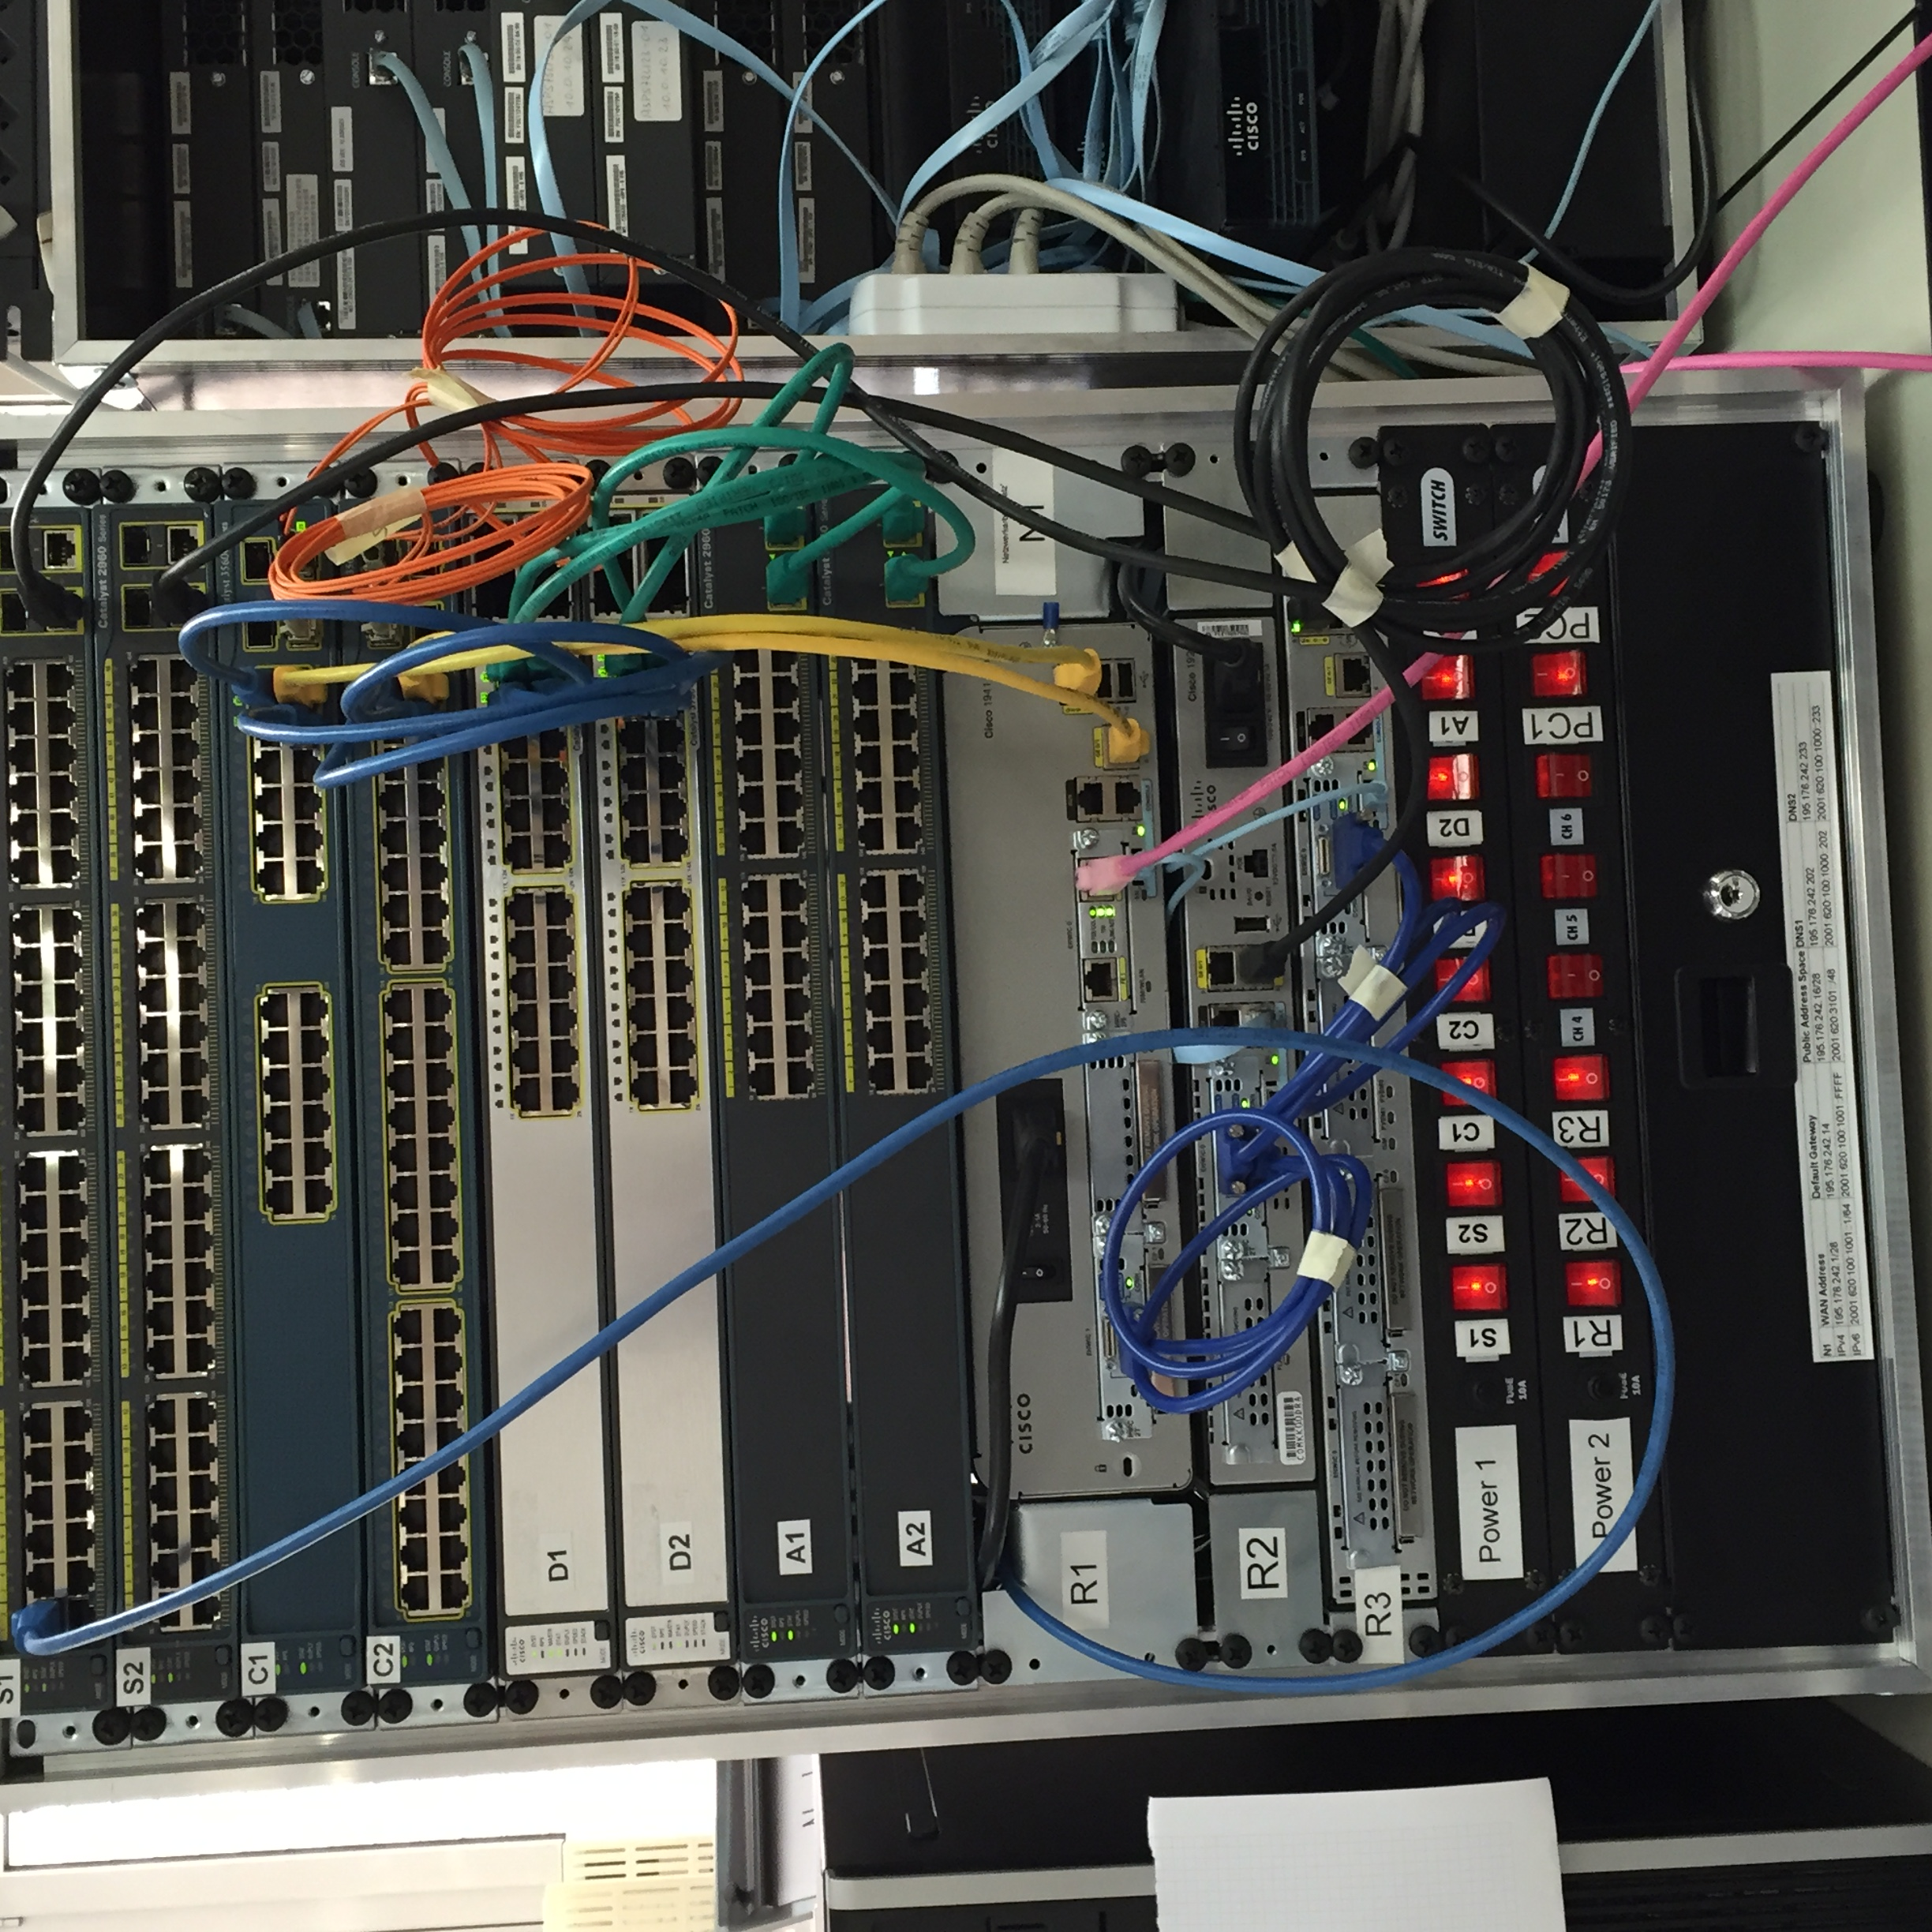
\includegraphics[angle=270,scale=0.1]{Hardware}
\caption{Hardware}
\label{abb:Hardware }
\end{figure}

\pagebreak

%--------Inhaltsverzeichnis---------- 
\tableofcontents 
\pagebreak

%--------Abbildungsverzeichnis----------
\listoffigures
\renewcommand*\clearpage{}

%--------Tabellenverzeichnis----------
%\listoftables 
%\renewcommand*\clearpage{}
%--------listings----------
\lstlistoflistings
\newpage



%--------Abkürzugsverzeichnis---------
\chapter{Abkürzungen}
\begin{acronym}[Bash]
\acro{ACL}{Access Control List}
\acro{DHCP}{Dynamic Host Configuration Protocol}
\acro{DNS}{Domain Name System}
\acro{LACP}{Link Aggreagtion Protocol}
\acro{NAT}{Network Address Translation}
\acro{PagP}{Port Aggregation Protocol}
\acro{RA}{Router Advertisement}
\acro{SLAAC}{Stateless Address Autoconfiguration}
\acro{VLAN}{Virtual Local Area Network}
\end{acronym}
\newpage


%--------Inhalt----------
\chapter{Ausgangslage} 
\section{Fallbeispiel}
Es soll ein neues Netzwerk für die Mittelgrosse Firma HAC Home Audio Center AG aufgebaut werden, welche 80 Mitarbeiter an den 3 Standorten Chur, Buchs, St. Gallen beschäftigt. Die Firma hat ihren Hauptsitz mit 70 Mitarbeitern in Chur und Niederlassungen mit je 5 Mitarbeitern in Buchs und St. Gallen. Die Standorte sind durch ein Layer-3 MPLS VPN miteinander verbunden (was durch einen einfachen Switch simuliert wird).
\newpage


\section{Praktikumsausrüstung} 
Die Netzwerkkomponenten sind bereits vorhanden, die physische Netzstruktur aufgrund der Gebäudetopographie und der Skalierbarkeit zu einem grossen Teil vorgegeben.\\
\newline
Die verfügbaren Komponenten sind:\\
\newline
-Standort Chur:\\
- 1x Router (Cisco 1941) mit 2x FastEthernet und 2x GigabitEthernet Anschlüssen\\
- 2x Layer-3 Switch (Cisco 3750E)\\
- 2x Layer-3 Switch (Cisco 3560G)\\
- 2x Layer-2 Switch (Cisco 2960)\\
\newline
-Standort Buchs:\\
- 1x Router (Cisco 1921)\\
- 1x Layer-2 Switch (Cisco 2960)\\
\newline
-Standort St.Gallen:\\
- 1x Router (Cisco 2901)\\
- 1x Layer-2 Switch (Cisco 2960)\\
\newline
Die vorgegebene Netzwerkstruktur ist in Abbildung \ref{abb: Netzwerksturktur} zu sehen:
\begin{figure} [H]
\centering
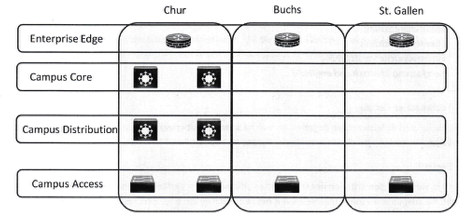
\includegraphics{Netzwerkstruktur.png}
\caption{Netzwerkstruktur}
\label{abb: Netzwerksturktur}
\end{figure}
\newpage

\chapter{Konzept}
In den Kapiteln \ref{ipv4} und \ref{ipv6} sind die IP-Konzepte beschrieben. In Abbildung \ref{abb: IP-Addressplan} ist die Verteilung der IP-Adressen aufgeführt.
\section{Ipv4 Adresskonzept} \label{ipv4}
Das folgende Konzept gilt nur für IPv4, immer wenn von Adressen die Rede ist, sind nur IPv4 Adressen gemeint.
Für das private Netz werden Adressen aus dem 10.0.0.0/8 Netz ausgewählt. Für jeden Standort und für die Netze welche nicht einem Standort zugeordnet werden können, wird ein /16 Netz ausgewählt, so hat jeder Standort 65534 Ip-Adressen. Dies sollte für die nahe Zukunft genügen.\\
\newline
Die Aufteilung sieht folgendermassen aus: \\
\newline
\hspace*{1cm} 
\begin{tabular}{ll}
    Chur & 10.\colorbox{green}{1}.0.0/16\\
    St. Gallen & 10.\colorbox{green}{2}.0.0/16\\
    Buchs & 10.\colorbox{green}{3}.0.0/16\\
    Transfer & 10.\colorbox{green}{4}.0.0/16\\
\end{tabular}\\
\newline
Für die \acs{VLAN}s werden die Netze der Standorte nochmals unterteilt, die gelben Sterne im \acs{VLAN}-Plan stehen für die Standorte. Mit /24 Netzen stehen jeder Abteilund pro Standort 256 Adressen zur Verfügung.\\
\newline
\hspace*{1cm} 
\begin{tabular}{lll}
     \acs{VLAN} 10 & Geschäftsleitung & 10.\colorbox{yellow}{*}.\colorbox{green}{10}.0/24\\
     \acs{VLAN} 20 & Buchhaltung & 10.\colorbox{yellow}{*}.\colorbox{green}{20}.0/24\\
     \acs{VLAN} 30 & Entwicklung & 10.\colorbox{yellow}{*}.\colorbox{green}{30}.0/24\\
             & Transfer & 10.\colorbox{yellow}{*}.\colorbox{green}{40}.0/24\\
     \acs{VLAN} 99 & Management & 10.\colorbox{yellow}{*}.\colorbox{green}{99}.0/24\\
\end{tabular}
\newpage
\section{Ipv6 Adresskonzept} \label{ipv6}
Das folgende Konzept gilt nur für IPv6, immer wenn von Adressen die Rede ist, sind nur IPv6 Adressen gemeint.
Die Aufgabenstellung besagt, dass ein /48 Netz zur Verfügung steht, das Ziel ist nun dies in einer ähnlichen Art wie bei IPv4 zu gestalten. \\
\newline
Standortabhängigkeiten:\\ 
\newline
\hspace*{1cm} 
\begin{tabular}{ll}
    Chur & 2001:620:3101:\colorbox{green}{1}::/64\\
    St. Gallen & 2001:620:3101:\colorbox{green}{2}::/64\\
    Buchs & 2001:620:3101:\colorbox{green}{3}::/64\\
\end{tabular}\\
\newline
Da es bei IPv6 keine \acs{VLAN}s gibt, sondern alles über Layer-3, sprich IP, geschieht. Muss auch ein “\acs{VLAN}-Konzept” für IPv6 erstellt werden. Dies wird analog zu IPv4 gemacht. Die gelben Sterne stehen für die Standortadresse.\\\newline
Netze der Abteilungen: \\
\newline
\hspace*{1cm} 
\begin{tabular}{lll}
     \acs{VLAN} 10 & Geschäftsleitung & 2001:620:3101:\colorbox{yellow}{*}\colorbox{green}{010}::/64\\
     \acs{VLAN} 20 & Buchhaltung & 2001:620:3101:\colorbox{yellow}{*}\colorbox{green}{020}::/64\\
     \acs{VLAN} 30 & Entwicklung & 2001:620:3101:\colorbox{yellow}{*}\colorbox{green}{030}::/64\\
             & Transfer & 2001:620:3101:\colorbox{yellow}{*}\colorbox{green}{040}::/64\\
     \acs{VLAN} 99 & Management & 2001:620:3101:\colorbox{yellow}{*}\colorbox{green}{099}::/64\\
\end{tabular}



\begin{figure} [H]
\centering
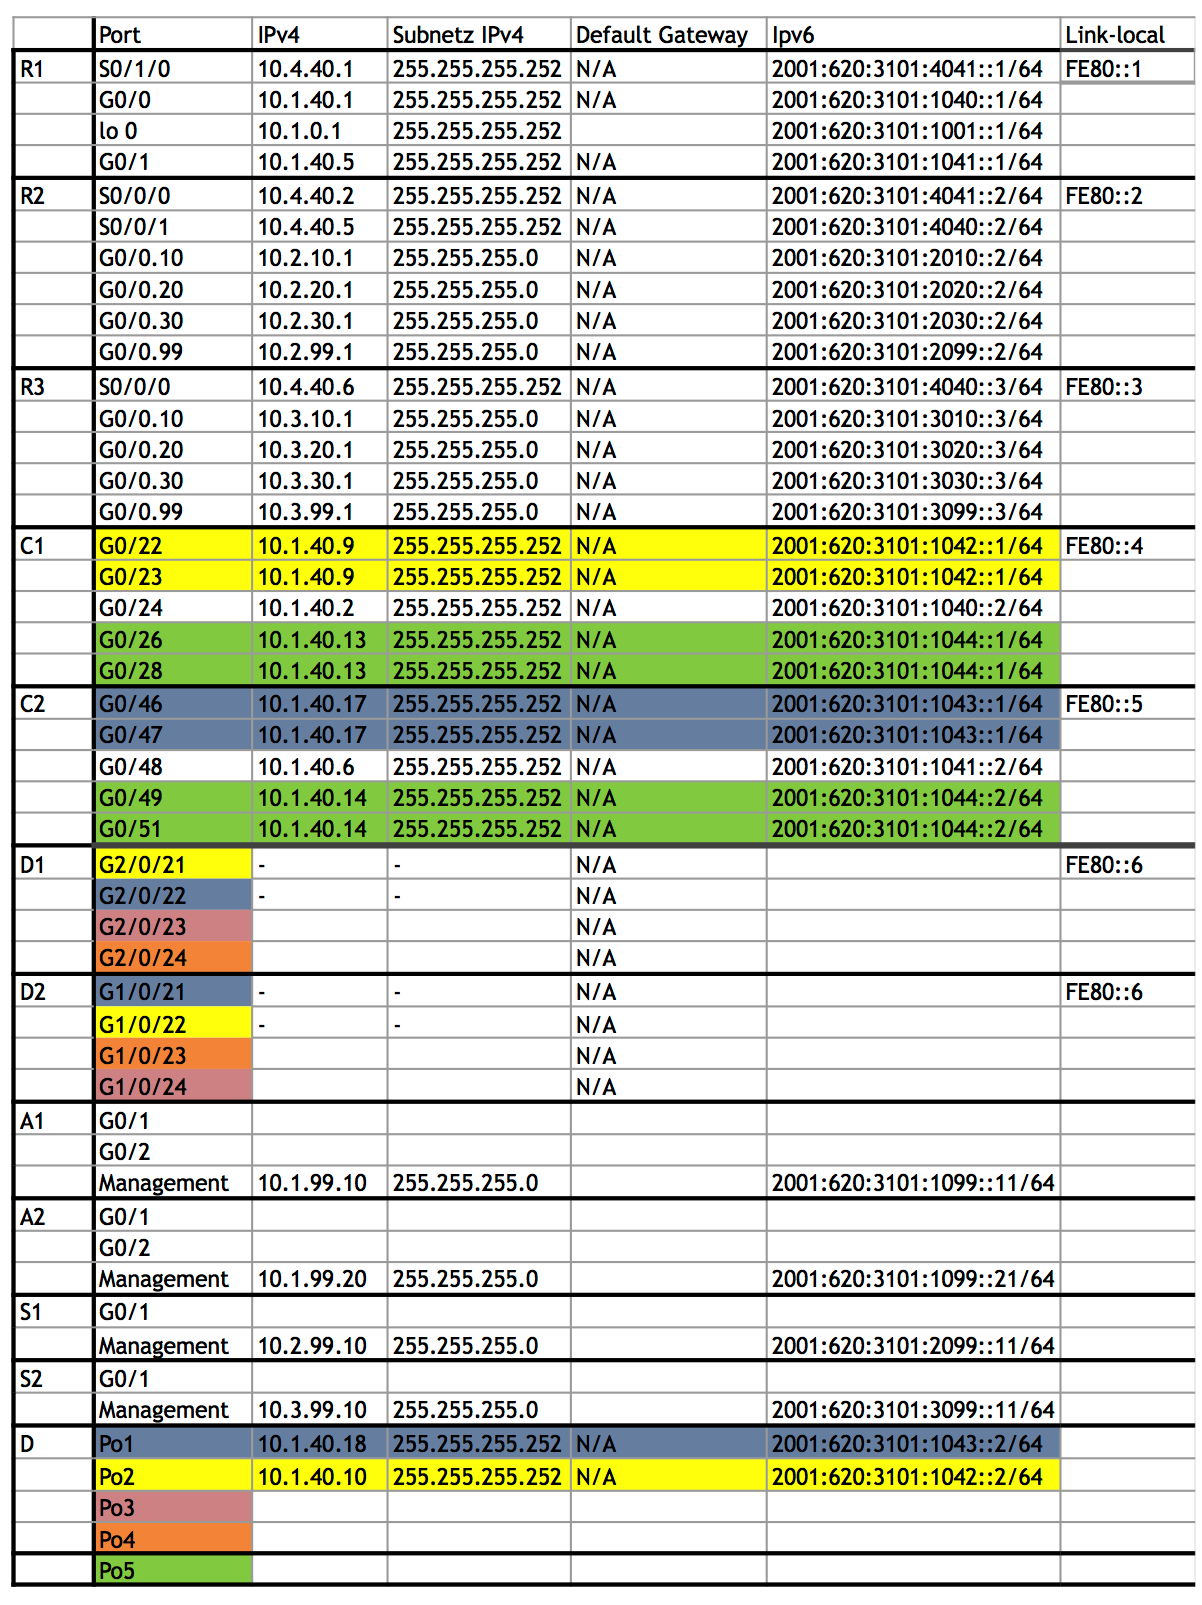
\includegraphics[angle=0,scale=0.4]{Iuk_III_U_addressplan.png}
\caption{IP-Addressplan}
\label{abb: IP-Addressplan}
\end{figure}


\section{Routingkonzept} 
Innerhalb unseres Unternehmens werden die verschiedenen Standorte miteinander über OSPF geroutet. Am Hauptstandort in Chur wird ab dem Distribution-Switch (D) ebenfalls mit OSPF geroutet. Beim Interface mit dem Internetanschluss wird eine default-Route gesetzt, da diese immer die Gleiche ist. Damit die Clients immer den gleichen default-Gateway haben, ist auf R1 noch ein Loopback-Interface erstellt worden, dieses darf nicht vergessen werden bei der Konfiguration von OSPF.

\section{NAT Konzept}
Meistens ist es für ein Unternehmen nicht rentabel sich die gesamte Anzahl benötigter IP-Adressen zu  kaufen. Deshalb werden private IP-Adressen verwendet und danach können mit einem \acs{NAT} ganze Subnetze zu einer öffentlichen Adresse zugeordnet werden. Dies ist eine komfortable Lösung, ausserdem können dann die privaten Adressen so gestaltet werden, dass man nur schon beim anschauen weiss, an welchem Standort und zu welchem \acs{VLAN} die Adresse gehört.

\subsection{IPv4}
Für die öffentlichen Adressen steht ein /28 Netz zur Verfügung. Für die Verwendung von \acs{NAT} können alle Adressen des Netzes benutzt werden, die Netz- und Broadcast-Adresse werden nicht benötigt. Somit stehen 16 öffentliche Adressen zur Benutzung, hier wurde für jeden \acs{VLAN} an jedem Standort eine eigene Adresse verteilt. Dies ergibt 12 Adressen, die restlichen 4 Adressen sind für Reserven eingeplant.

\subsection{IPv6}
Bei IPv6 ist kein \acs{NAT} notwendig, da ein öffentliches /48 Netz gebraucht wird. Es sind also mehr Adressen vorhanden als je in diesem Kleinunternehmen gebraucht werden.

\newpage
\section{Securitykonzept} 
\subsection{ACL} \label{acl}
Mit \acs{ACL}'s wird der Zugriff der Abteilungen untereinander verhindert, lediglich das Management-\acs{VLAN} hat auf alles Zugriff, da dies für die reibungslose Verwaltung des Netzes erforderlich ist.
Die \acs{ACL}'s werden auf den Routern R2, R3 und auf dem Switch D konfiguriert, für die 3 \acs{VLAN}s der Abteilungen wird je der Zugriff der anderen \acs{VLAN}s verboten, danach werden alle anderen IP und TCP Pakete erlaubt. Dies wird für IPv4 und IPv6 gleich gemacht, als erstes wird eine ACL pro \acs{VLAN} erstellt, danach wird diese \acs{ACL} dem \acs{VLAN}-Interface zugewiesen.

\subsection{Layer 2 Security}
Leider konnte das Layer 2 Sicherheitskonzept aufgrund von zeitlichen Verzögerungen nicht umgesetzt werden. Folgende Punkte waren als Sicherheitsmassnahmen gedacht: 
\begin{itemize}
\item Port Security: Um MAC-Spoofing zu verhindern, wird ein Interface fest mit einer MAC-Adresse verknüpft, dies geschieht mit der Konfiguration von Port Security.
\item Ports abschalten: Alle nicht aktiven Ports down schalten, so kann nicht irgendwer sein Gerät einstecken und Unfug treiben.
\item Trunk: Auf den Trunkports sollen nur die \acs{VLAN}s zugelassen werden, welche auch effektiv gebraucht werden.
\end{itemize}

\newpage
\section{Serverservices}
\subsection{IPv4}
\acs{DHCP} wird auf dem Router R1 konfiguriert. Dazu wird pro Standort und \acs{VLAN} ein Pool eingerichtet. Ein Pool beinhaltet jeweils das Netz, von welchem IP-Adressen vergeben werden, die \acs{DNS}-Server und den Default-Router. Weiter werden auf dem Distribution-Switch und den Routern R1 und R2 noch Relays eingerichtet.
\subsection{IPv6}
Bei IPv6 werden die Adressen via \acs{SLAAC} vergeben. Um allerdings das Internet nutzen zu können muss der \acs{DNS}-Server bekannt sein. Dafür muss auf dem Router R1 ein \acs{DHCP}-Pool erstellt werden und den Interfaces zugewiesen werden. Weiter muss auf den Interfaces der Router das \acs{RA}-Flag gesetzt werden. Um eine schnelle Verteilung der IPv6 Adressen 
zu erreichen, wird das \acs{RA}-Intervall eingestellt werden. Damit auch die Router R2 und R3 den \acs{DHCP}-Pool erreichen können muss auf den Interfaces ein Relay eingerichtet werden.
\section{Netzwerkplan}

\begin{figure} [H]
\centering
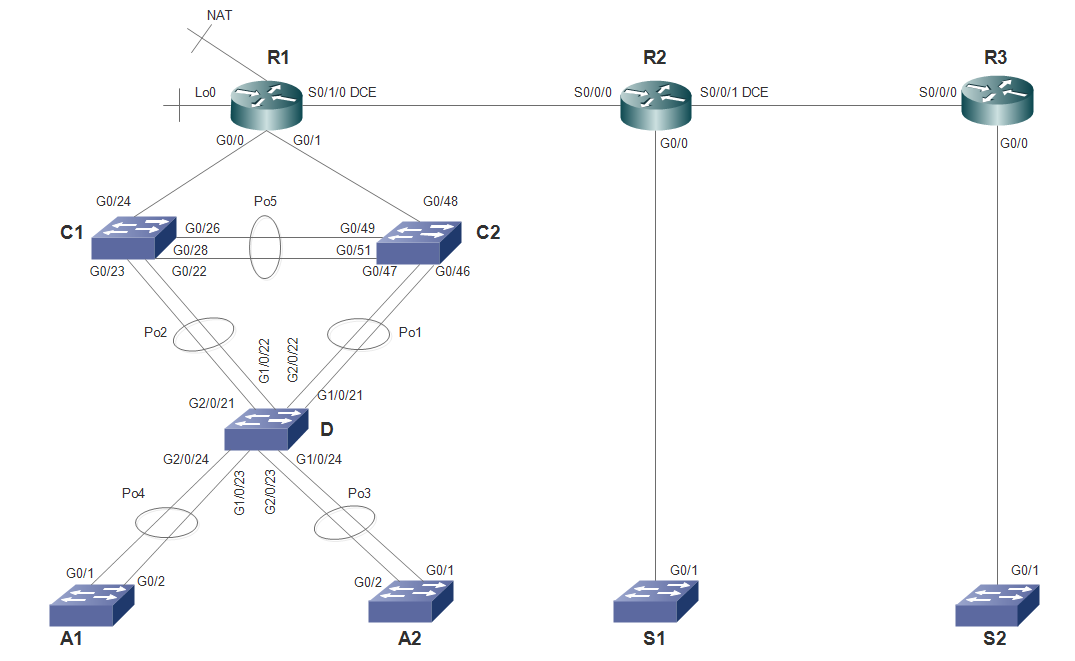
\includegraphics[angle=0,scale=0.43]{Netzwerkplan}
\caption{Netzwerkplan}
\label{abb: Netzwerkplan}
\end{figure}
\newpage


\section{Weitere Überlegungen}

Bei genügender Zeit hätte man noch einiges erreichen können. Einige Punkte welche wichtig sind werden nun erläutert:
\begin{itemize}
\item Passwort setzen: Im Moment ist auf keinem Gerät ein Passwort gesetzt, da es während der Konfiguration mühsam ist immer wieder das Passwort einzugeben, deshalb sollte dies ganz am Schluss geschehen.
\item Fernwartung: Auf allen Geräten ist eine Management Adresse konfiguriert. Wenn jetzt der Fernzugriff aktiviert würde, müssten die Anzahl Zugriffe aus dem Internet begrenzt werden, damit nicht mit Bruteforce das Passwort geknackt werden kann.
\item OSPF Areas: Die einzelnen Standorte hätten noch mit einem eigenen OSPF Area konfiguriert werden können, dies hätte den Vorteil dass nicht alle OSPF Teilnehmer über das ganze Netz bescheid wissen müssen und so bedeutend weniger Traffic auf den Leitungen ist.
\item \acs{VLAN}: Es hätte noch ein Gäste\acs{VLAN} eingerichtet werden können, welches nur zum Internet zugriff hat, dies ist jedoch nicht Teil der Aufgabenstellung und könne im Bedarfsfall schnell nachgerüstet werden.
\item Device Backups: Wenn im Moment Device Backups gemacht werden müssen, muss jeder einzelne Router und Switch mittels kopieren der running-config gebackupt werden. Dabei könnte man mit einem Kron-Script die Backups zeitgesteuert auf einen TFTP Server speichern. So spart man sich wöchentliche Arbeit und man vergisst es auch sicher nicht.
\end{itemize}

\section{Stack}
Stacken ist das Zusammenschliessen zweier physischen Switches zu einem logischen. Dies ist nicht mit allen Switches möglich, doch in diesem Fall ist es bei den Beiden Distribution-Switches möglich, da diese ein Stack-Interface auf der Rückseite haben. Dies erspart eine Menge an Arbeit, wenn man weiss wie dies funktioniert. In diesem Fall war dies leider nicht der Fall, da noch nie mit gestackten Switches gearbeitet wurde, die Anweisungen zur Konfiguration des Stackes bezieht sich hier nur auf die Cisco Catalyst 3750 Switches, da nicht bekannt ist ob es noch Besonderheiten bei der Konfiguration anderer Switches gibt. Das gröste Problem war, dass der 3750er nur \acs{LACP} und kein \acs{PagP} unterstützt.


\newpage
\chapter{Planung}
In Abbildung \ref{abb:Zeitplan} ist der geplante und der tatsächliche Ablauf des Projektes zu sehen. 
\begin{figure}[H]
\begin{center}
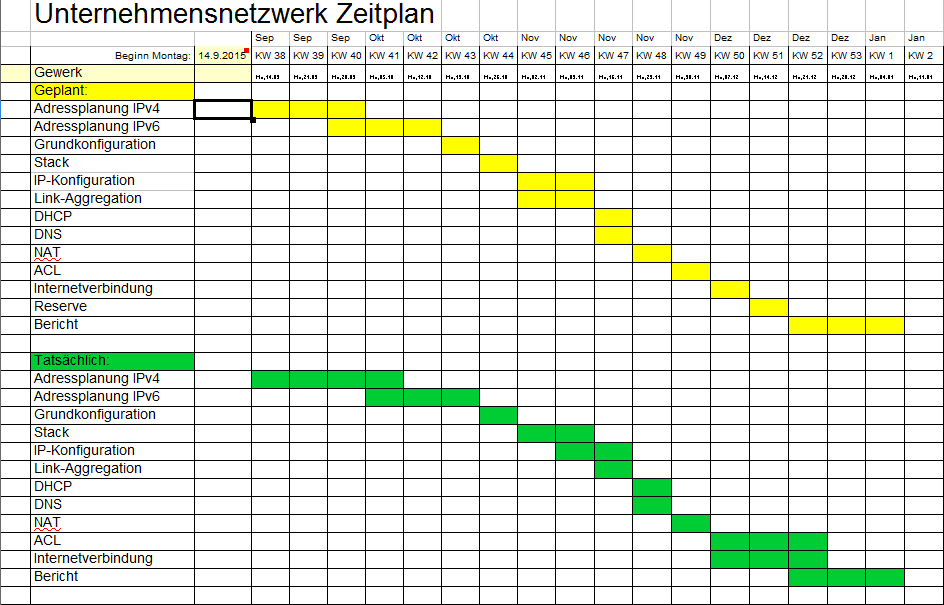
\includegraphics[angle=90,scale=0.52]{Zeitplan.png}
\caption{Zeitplan}
\label{abb:Zeitplan}
\end{center}
\end{figure}

\chapter{Umsetzung}


\section{Grundlegende Konfiguration Router}

 \begin{lstlisting}[frame=single, captionpos=b,caption= Router Grundkonfiguration]
R1(config)#hostname R1
R1(config)#no ip domain lookup
R1(config)#ipv6 unicast-routing
\end{lstlisting}

\section{Grundlegende Konfiguration Access-Switches}
Da auf den Access-Switches das Default Template kein IPv6 unterstützt, muss zuerst das Template gewechselt werden, um IPv6 nutzen zu können. Nach dem Template Wechsel ist ein Neustart des Switches nötig. Der Template Wechsel wird wie folgt durchgeführt:
\newline

\begin{lstlisting}[frame=single, captionpos=b,caption= Switch Template Wechsel]
Switch(config)#sdm prefer dual-ipv4-and-ipv6 default
Switch(config)#reload
\end{lstlisting}
\noindent
Danach kann die Grundkonfiguration vorgenommen werden. Das Default-Gateway ist die jeweilige IP-Adresse des Management \acs{VLAN}s des jeweiligen Routers oder Distribution-Switches.
\newline

\begin{lstlisting}[frame=single, captionpos=b,caption= Switch Grundkonfiguration]
S1(config)#hostname A1
S1(config)#no ip domain lookup
S1(config)#spanning-tree mode pvst
S1(config)#ip default-gateway 10.2.99.1
\end{lstlisting}
\newpage
\section{IP-Konfiguration}
\subsection{Router}
Auf den Routern wurde auf das jeweilige GigabitEthernet-Interface die dazugehörige IPv4 und IPv6 Adresse zugewiesen. Zusätzlich wurde pro Router noch eine Link-Local Adresse zugewiesen, welche jedem genutztem GigabitEthernet-Interface zugewiesen werden muss. Des Weiteren muss auf dem Interface noch IPv6 aktiviert werden.
Auf den Routern R2 und R3 werden die Konfigurationen auf den Subinterfaces vorgenommen.
\newline
\begin{lstlisting}[frame=single, captionpos=b,caption= Router IP-Konfiguration]
R1(config)#interface GigabitEthernet0/0
R1(config-if)#ip address 10.1.40.1 255.255.255.252
R1(config-if)#ipv6 address FE80::1 link-local
R1(config-if)#ipv6 address 2001:620:3101:1040::1/64
R1(config-if)#ipv6 enable
\end{lstlisting}

\subsection{Distribution-Switch}
Auf den Distribution-Switches wird gleich wie bei den Routern vorgegangen, allerdings werden die IP-Adressen, wenn vorhanden, auf den Port-Channel konfiguriert (siehe Kapitel \ref{linkaggre}). Zusätzlich müssen hier noch die \acs{VLAN}-Interfaces mit den zugehörigen IP-Adressen definiert werden.
\newline
\begin{lstlisting}[frame=single, captionpos=b,caption= Distribution IP-Konfiguration]
D(config)#interface VLAN 10
D(config-if)#description Geschaeftsleitung
D(config-if)#ip address 10.1.10.1 255.255.255.0
D(config-if)#ipv6 address FE80::6 link-local
D(config-if)#ipv6 address 2001:620:3101:1010::1/64
D(config-if)#ipv6 enable
\end{lstlisting}

\subsection{Access-Switches}
Auf den Acces-Switches wird eine IP-Adresse dem Management-\acs{VLAN} zugewiesen.
\newline
\begin{lstlisting}[frame=single, captionpos=b,caption= Access-Switch IP-Konfiguration]
interface VLAN 99
 ip address 10.1.99.10 255.255.255.0
 ipv6 address 2001:620:3101:1099::11/64
\end{lstlisting}

\section{Link-Aggregation} \label{linkaggre}
Bei der Konfiguration der Port-Channel war wichtig das zuerst der Port-Channel selbst definiert wird und erst danach die Zuweisung zum GigabitEthernet-Interface erfolgt. Des Weiteren war darauf zu achten das sowohl der Port-Channel als auch das GigabitEthernet-Interface als no Switchport definiert wurden, sofern dies erwünscht ist.
\newline
\begin{lstlisting}[frame=single, captionpos=b,caption= Switch Grund Konfiguration]
D(config)#interface Port-channel1
D(config-if)#no switchport
D(config-if)#ip address 10.1.40.18 255.255.255.252
D(config-if)#ipv6 address FE80::6 link-local
D(config-if)#ipv6 address 2001:620:3101:1043::2/64
D(config-if)#ipv6 enable
D(config)#interface GigabitEthernet2/0/22
D(config-if)#no switchport
D(config-if)#no ip address
D(config-if)#channel-group 1 mode active
\end{lstlisting}

\section{OSPF}
\subsection{IPv4}
In Listing \ref{ospfipv4} ist die OSPF Konfiguration für IPv4 zu sehen. Dabei werden die angrenzenden Netzadressen angegeben. Access-Ports werden als Passive-Interface konfiguriert damit sie keine Hello-Packets empfangen.
\newline
\begin{lstlisting}[frame=single, captionpos=b,caption= OSPF IPv4, label=ospfipv4]
R2(config)#router ospf 1
R2(config-router)#passive-interface GigabitEthernet0/0.10
R2(config-router)#passive-interface GigabitEthernet0/0.20
R2(config-router)#passive-interface GigabitEthernet0/0.30
R2(config-router)#passive-interface GigabitEthernet0/0.99
R2(config-router)#network 10.2.10.0 0.0.0.255 area 0
R2(config-router)#network 10.2.20.0 0.0.0.255 area 0
R2(config-router)#network 10.2.30.0 0.0.0.255 area 0
R2(config-router)#network 10.2.99.0 0.0.0.255 area 0
R2(config-router)#network 10.4.40.0 0.0.0.3 area 0
R2(config-router)#network 10.4.40.4 0.0.0.3 area 0
\end{lstlisting}

\subsection{IPv6}
Bei IPv6 erfolgt die Konfiguration auf den einzelnen Interfaces.
\newline
\begin{lstlisting}[frame=single, captionpos=b,caption= OSPF IPv6]
R2(config)#interface GigabitEthernet0/0.10
R2(config-if)#ipv6 ospf 1 area 0
\end{lstlisting}
\section{NAT}
\acs{NAT} wird auf dem Router R1 konfiguriert. Hierzu werden die einzelnen Interfaces als ip \acs{NAT} outside oder inside konfiguriert. Zusätzlich werden noch pro \acs{VLAN} und Standort \acs{NAT}-Pools und \acs{ACL}'s definiert welche dann dem \acs{NAT} zugewiesen werden. In Listing \ref{nat} sind die \acs{NAT}-Pools und \acs{ACL}'s für das \acs{VLAN} 10 definiert.
\newline
\begin{lstlisting}[frame=single, breaklines=true, captionpos=b,caption= \acs{NAT},label=nat ]
R1(config)#interface FastEthernet0/0/0
R1(config-if)#ip nat outside
R1(config)#interface GigabitEthernet0/0
R1(config-if)#ip nat inside
R1(config)#interface GigabitEthernet0/1
R1(config-if)#ip nat inside
R1(config)#interface Serial0/1/0
R1(config-if)#ip nat inside
R1(config)#ip nat pool chur10 195.176.242.17 195.176.242.17 netmask 255.255.255.240
R1(config)#ip nat pool buchs10 195.176.242.21 195.176.242.21 netmask 255.255.255.240
R1(config)#ip nat pool stgallen10 195.176.242.25 195.176.242.25 netmask 255.255.255.240
R1(config)#access-list 101 permit ip 10.1.10.0 0.0.0.255 any
R1(config)#access-list 105 permit ip 10.2.10.0 0.0.0.255 any
R1(config)#access-list 109 permit ip 10.3.10.0 0.0.0.255 any
R1(config)#ip nat inside source list 101 pool chur10 overload
R1(config)#ip nat inside source list 105 pool buchs10 overload
R1(config)#ip nat inside source list 109 pool stgallen10 overload
\end{lstlisting}
\newpage

\section{ACL}
Die Access-Listen werden wie in Kapitel \ref{acl} beschrieben konfiguriert und einem Interface zugewiesen. In Listing \ref{aclconf} ist die Konfiguration von R2 für das \acs{VLAN} 10 zu sehen.
\newline
\begin{lstlisting}[frame=single, breaklines=true, captionpos=b,caption= ACL,label=aclconf]
R2(config)#interface GigabitEthernet0/0.10
R2(config-if)#ip access-group 116 in
R2(config-if)#ipv6 traffic-filter b10 in

R2(config)#access-list 116 deny   ip 10.2.10.0 0.0.0.255 10.1.20.0 0.0.0.255
R2(config)#access-list 116 deny   ip 10.2.10.0 0.0.0.255 10.1.30.0 0.0.0.255
R2(config)#access-list 116 deny   ip 10.2.10.0 0.0.0.255 10.2.20.0 0.0.0.255
R2(config)#access-list 116 deny   ip 10.2.10.0 0.0.0.255 10.2.30.0 0.0.0.255
R2(config)#access-list 116 deny   ip 10.2.10.0 0.0.0.255 10.3.20.0 0.0.0.255
R2(config)#access-list 116 deny   ip 10.2.10.0 0.0.0.255 10.3.30.0 0.0.0.255
R2(config)#access-list 116 permit ip any any
R2(config)#access-list 116 permit tcp any any

R2(config)#ipv6 access-list b10
R2(config-ipv6-acl)#deny ipv6 2001:620:3101:2010::/64 2001:620:3101:1020::/64
R2(config-ipv6-acl)#deny ipv6 2001:620:3101:2010::/64 2001:620:3101:1030::/64
R2(config-ipv6-acl)#deny ipv6 2001:620:3101:2010::/64 2001:620:3101:2020::/64
R2(config-ipv6-acl)#deny ipv6 2001:620:3101:2010::/64 2001:620:3101:2030::/64
R2(config-ipv6-acl)#deny ipv6 2001:620:3101:2010::/64 2001:620:3101:3020::/64
R2(config-ipv6-acl)#deny ipv6 2001:620:3101:2010::/64 2001:620:3101:3030::/64
R2(config-ipv6-acl)#permit ipv6 any any
R2(config-ipv6-acl)#permit tcp any any
\end{lstlisting}
\newpage

\section{DHCP \& DNS}
\acs{DHCP} und \acs{DNS} werden auf dem Router R1 Konfiguriert.
\subsection{IPv4}
Es wird pro Standort und \acs{VLAN} ein Adress-Pool definiert. Im Listing \ref{dhcpipv4} ist der Adress-Pool für das \acs{VLAN}10 des Standortes Chur definiert.
\newline
\begin{lstlisting}[frame=single, breaklines=true, captionpos=b,caption= IPv4 \acs{DHCP}, label=dhcpipv4]
R1(config)#ip dhcp pool C_10
R1(dhcp-config)#network 10.1.10.0 255.255.255.0
R1(dhcp-config)#dns-server 195.176.242.202 195.176.242.233
R1(dhcp-config)#default-router 10.1.10.1
\end{lstlisting}
\noindent
Des Weiteren werden auf dem Distribution-Switch, den Routern R2 und R3 noch ein DHCP-Relay konfiguriert. In Listing \ref{dhcpipv4relay} wird das Relay auf einem Interface von R2 Konfiguriert.
\newline
\begin{lstlisting}[frame=single, breaklines=true, captionpos=b,caption= IPv4 \acs{DHCP}-relay, label=dhcpipv4relay]
R1(config)#interface GigabitEthernet0/0.10
R1(config-if)#ip helper-address 10.1.0.1
\end{lstlisting}



\subsection{IPv6}
Für IPv6 muss auf R1 ein Pool eingerichtet werden, der den \acs{DNS}-Server 
beinhaltet.
\newline
\begin{lstlisting}[frame=single, breaklines=true, captionpos=b,caption= IPv6 \acs{DHCP}, label=dhcpipv6]
R1(config)#ipv6 dhcp pool pool
R1(config-if)# dns-server 2001:620:100:1000::202
\end{lstlisting}

\noindent
Auf den jeweiligen Interfaces der Routern muss für IPv6 noch das Flag gesetzt werden und es wird das Intervall der Router Advertisements eingestellt. Auf den Routern R2 und R3 muss noch das Relay gesetzt werden.
\newline
\begin{lstlisting}[frame=single, breaklines=true, captionpos=b,caption= IPv6 \acs{DHCP}-relay, label=dhcpipv6relay]
R2(config)#interface GigabitEthernet0/0.10
R2(config-if)#ipv6 nd other-config-flag
R2(config-if)# ipv6 nd ra interval 10
R2(config-if)#ipv6 dhcp relay destination 2001:620:3101:1001::1 Serial0/0/0
\end{lstlisting}
 




\newpage
\chapter{Fazit}
Wir taten uns am Anfang schwer mit dem Start und dem Addresskonzept. Als wir das Adresskonzept aufgestellt hatten, folgten weitere Probleme welche nicht zuletzt aufgrund der gestackten Switches auftraten, was zu Zeitverzögerungen führte. Dies ist auch auf dem Zeitplan in Abbildung \ref{abb:Zeitplan} zu sehen. Alles in Allem sind wir aber zufrieden dass wir uns für die gestackte Variante entschieden haben und so mal etwas anderes sehen konnten, was im Unterricht noch nicht vorgekommen ist. Ein weiteres Problem stellte die Organisation mit GitHub dar, dies weil wir nicht die aktuelle Konfiguration auf GitHub geladen haben sondern einfach immer die neuen Konfigurations Befehle ergänzt hatten, was dazu führte das Befehle vorhanden waren, die gar nicht existieren. Deshalb haben wir zum Schluss auch noch die aktuellen Konfigurationen der Switches ausgelesen und so weiterbearbeitet, was für kommende Projekte erneut so gemacht werden sollte. Die Verwaltung mit GitHub an sich war jedoch eine gefreute Sache und man konnte sich immer mal eine alte Version zurückholen. Schlussendlich sind wir auch zufrieden, da unser Netzwerk soweit funktioniert, das die grundlegenden Funktionen wie DHCP, Internetverbindung mit IPv4/IPv6 und die Verbindung zwischen den einzelnen Standorten innerhalb eines \acs{VLAN}s funktionieren.

%-----Anhang
\appendix
\addchap{Anhang}
\refstepcounter{chapter}

\section{R1}
\vspace{-1cm}
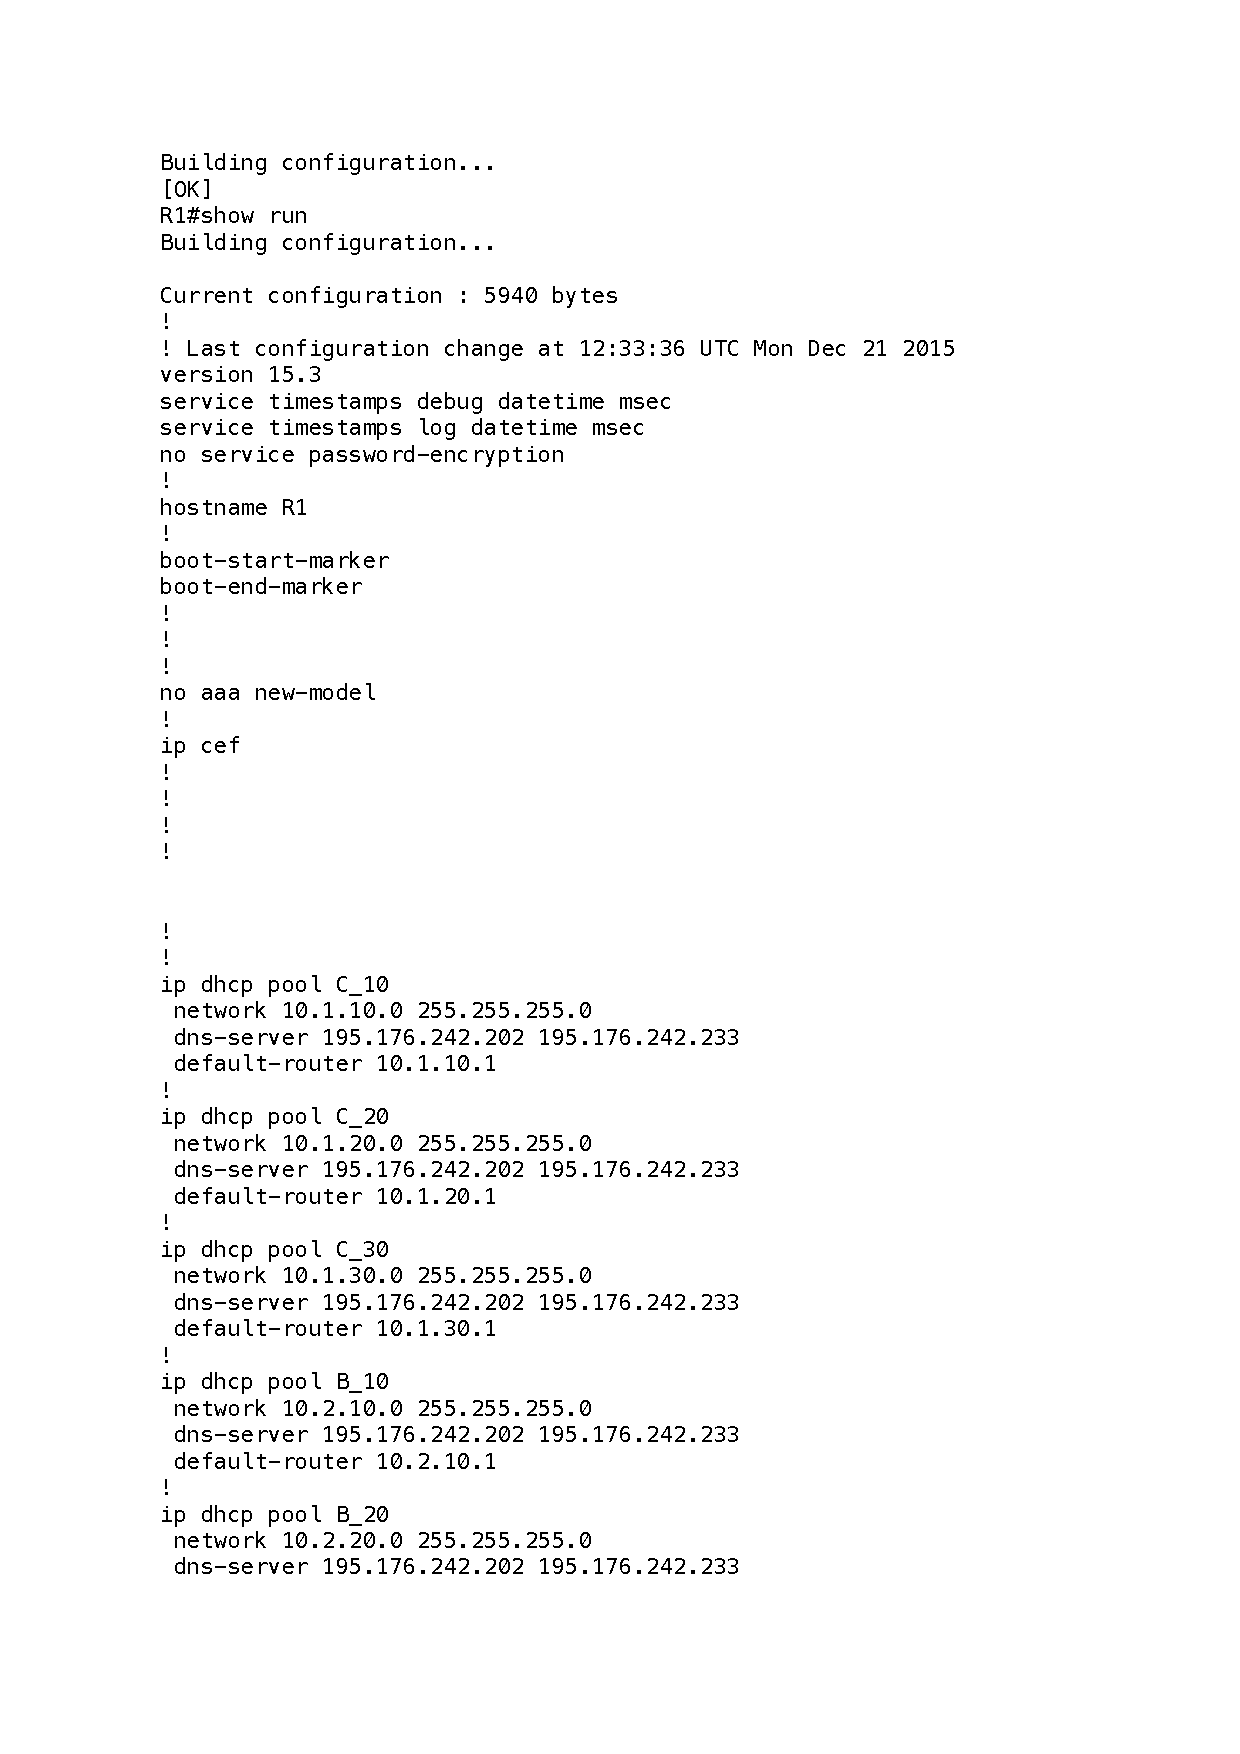
\includegraphics[height=\dimexpr\textheight-4\baselineskip\relax,page=1]{../config_files/R1.pdf}
\includepdf[pagecommand={\thispagestyle{headings}},pages=2-]{../config_files/R1.pdf}

\section{R2}
\vspace{-1cm}
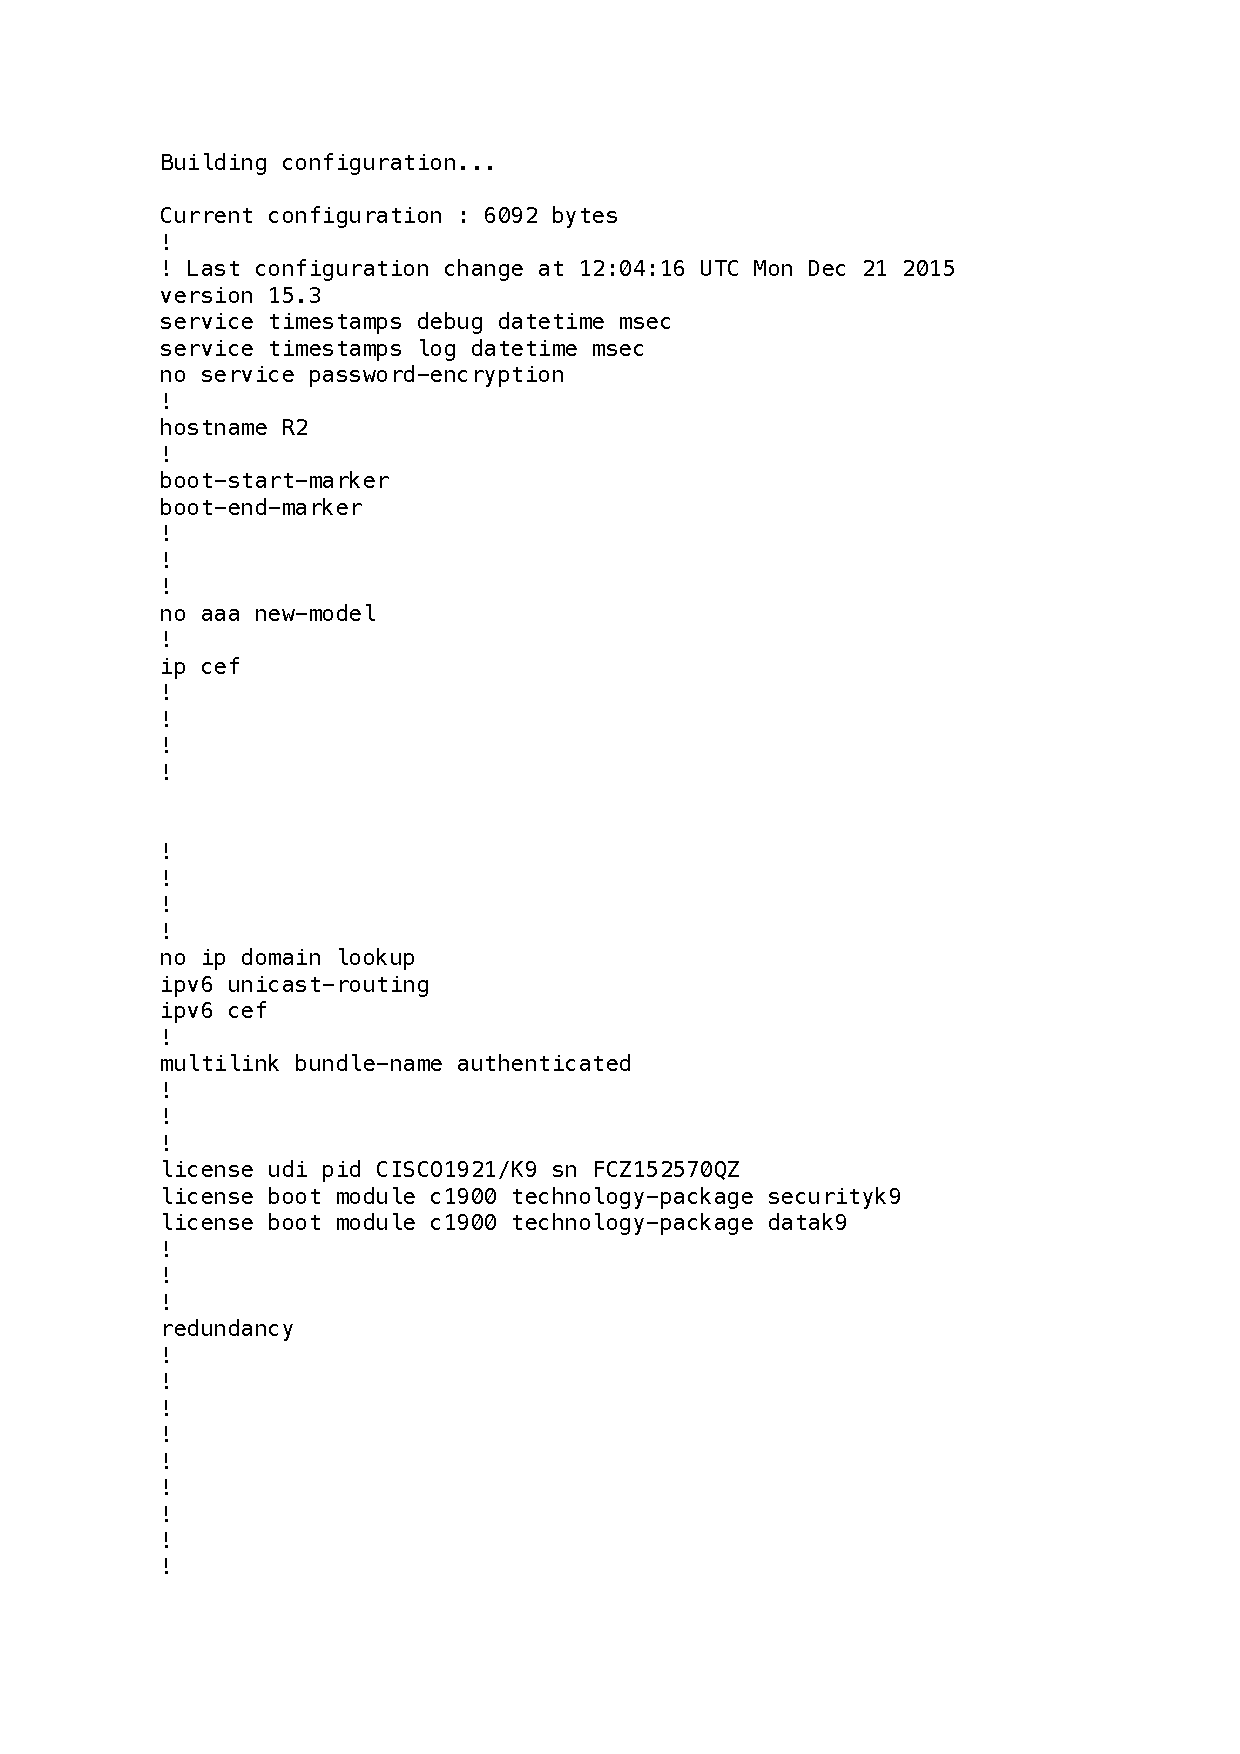
\includegraphics[height=\dimexpr\textheight-4\baselineskip\relax,page=1]{../config_files/R2.pdf}
\includepdf[pagecommand={\thispagestyle{headings}},pages=2-]{../config_files/R2.pdf}

\section{R3}
\vspace{-1cm}
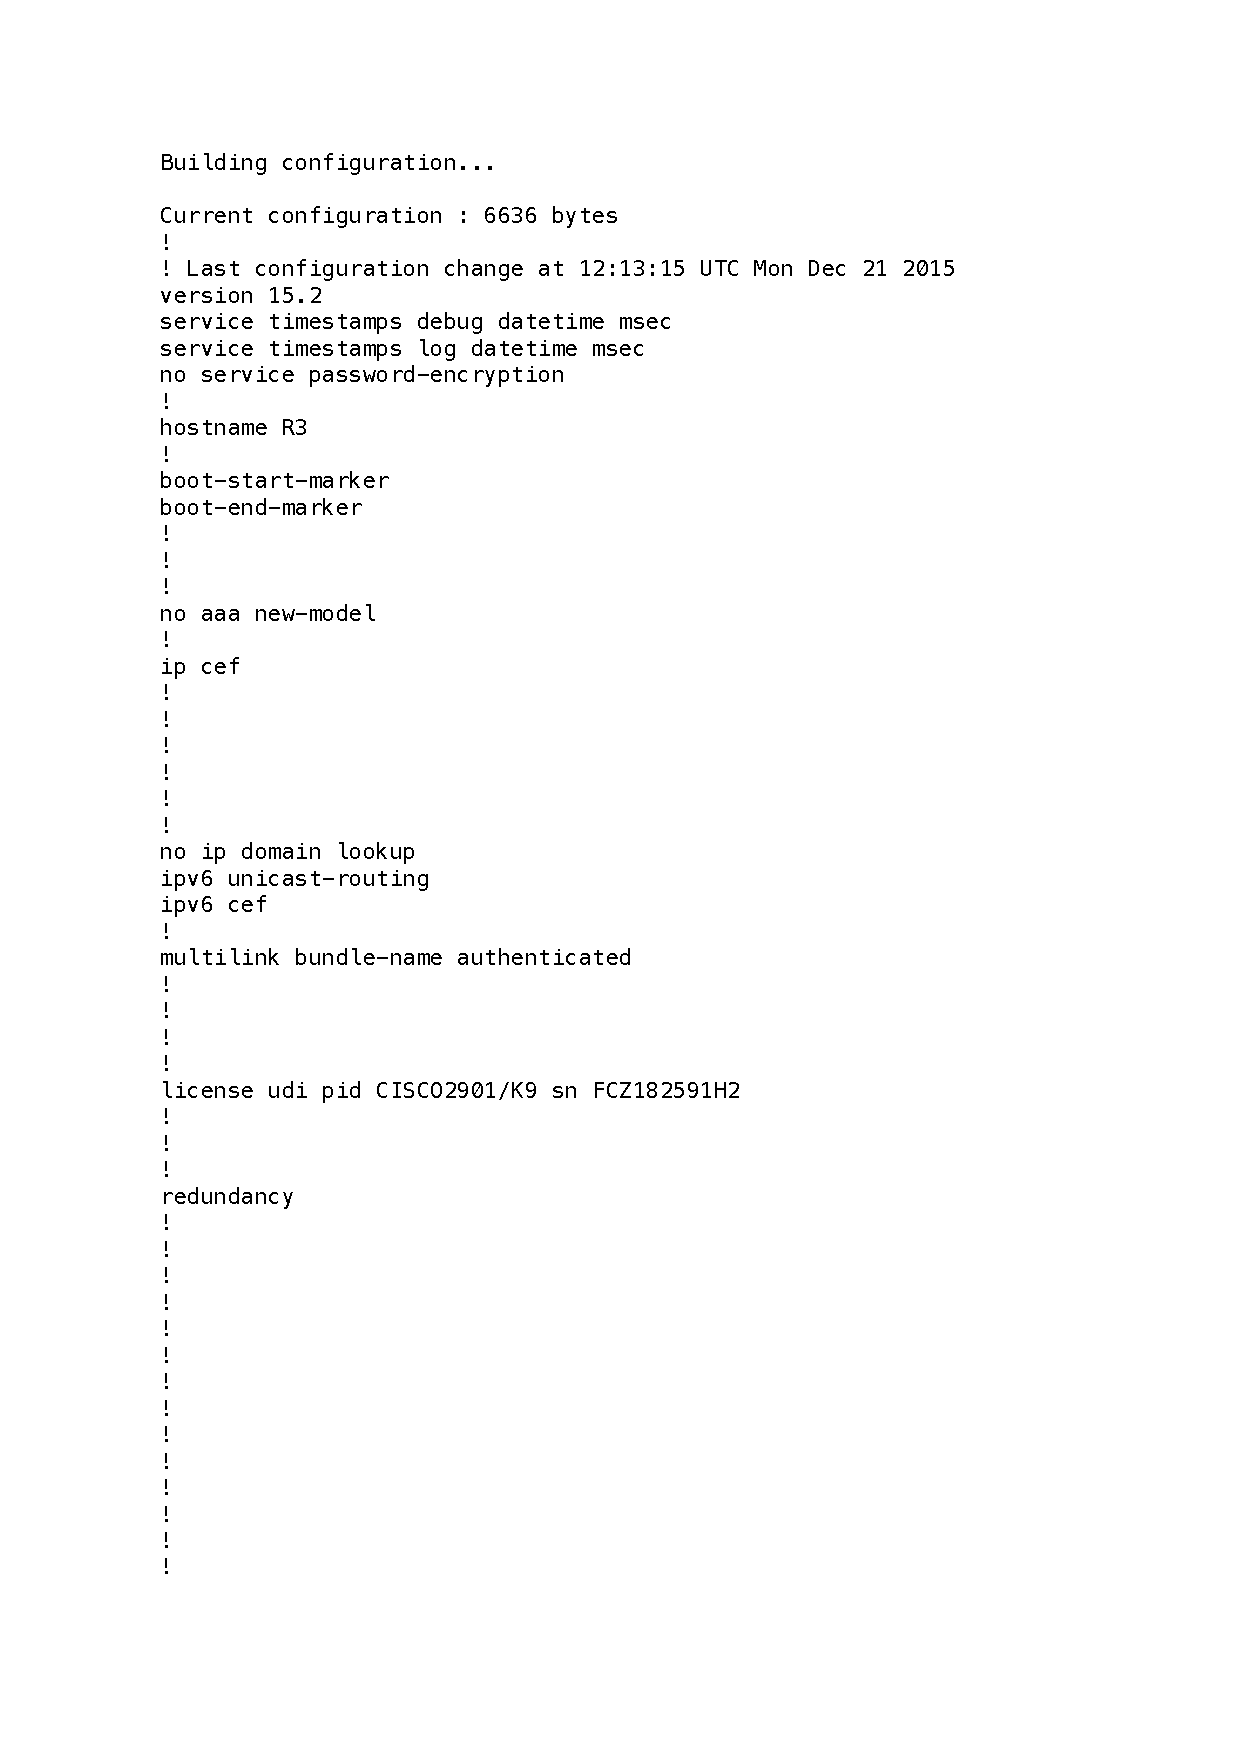
\includegraphics[height=\dimexpr\textheight-4\baselineskip\relax,page=1]{../config_files/R3.pdf}
\includepdf[pagecommand={\thispagestyle{headings}},pages=2-]{../config_files/R3.pdf}

\section{C1}
\vspace{-1cm}
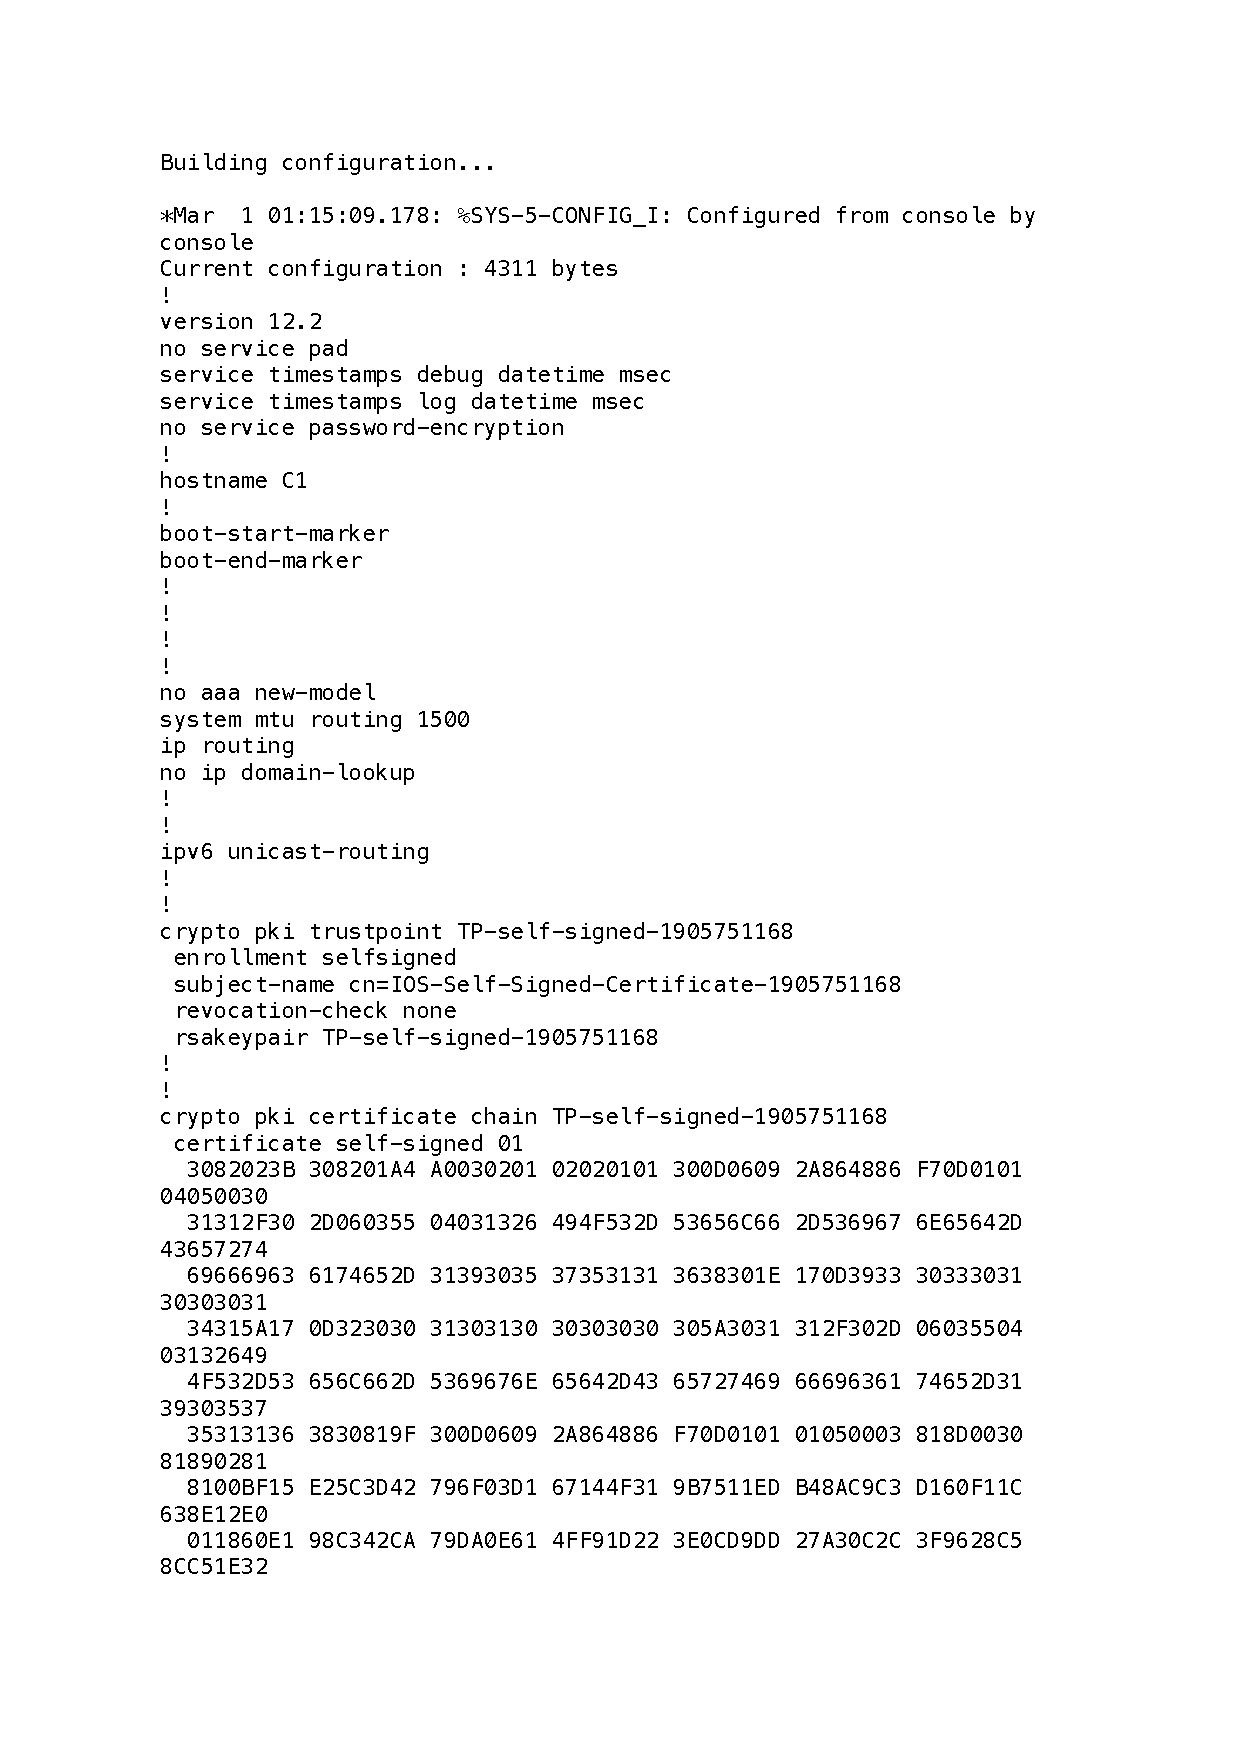
\includegraphics[height=\dimexpr\textheight-4\baselineskip\relax,page=1]{../config_files/C1.pdf}
\includepdf[pagecommand={\thispagestyle{headings}},pages=2-]{../config_files/C1.pdf}

\section{C2}
\vspace{-1cm}
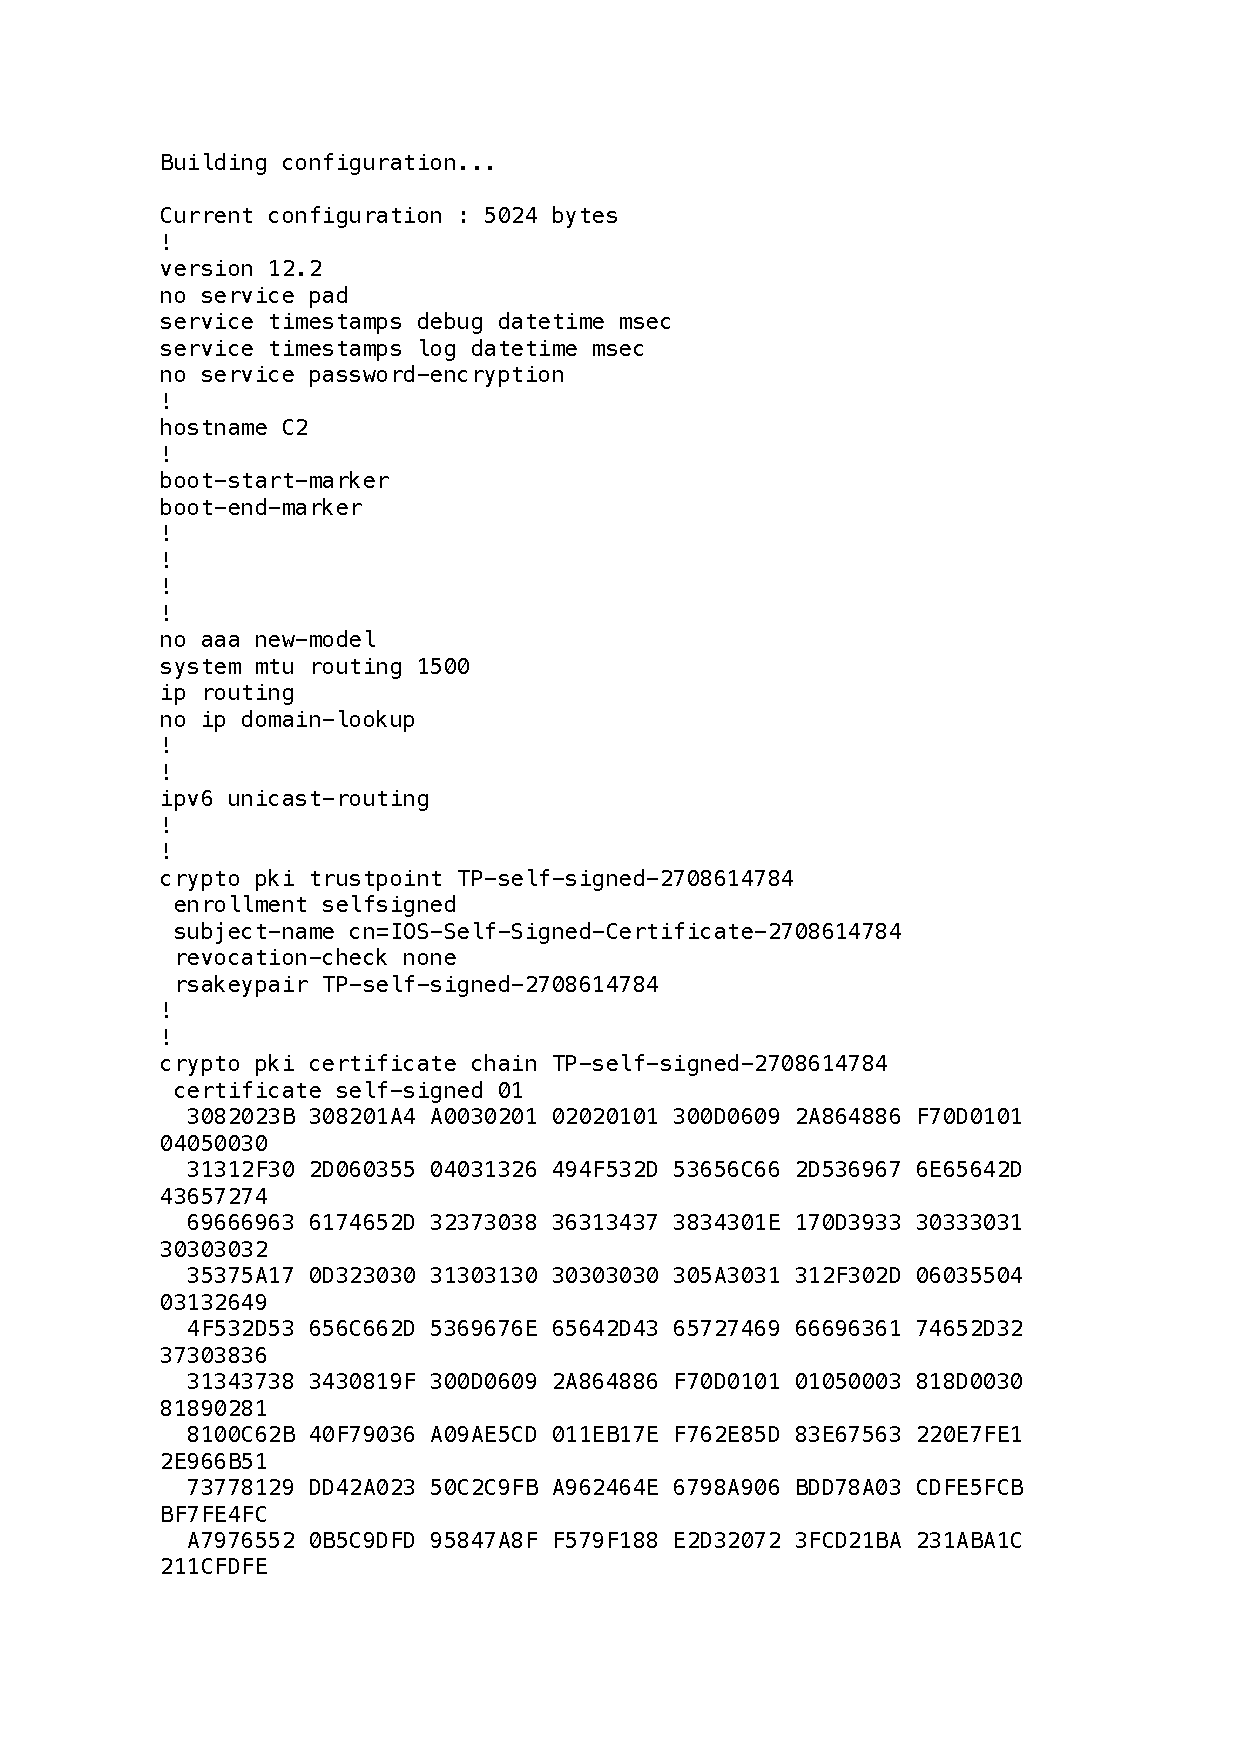
\includegraphics[height=\dimexpr\textheight-4\baselineskip\relax,page=1]{../config_files/C2.pdf}
\includepdf[pagecommand={\thispagestyle{headings}},pages=2-]{../config_files/C2.pdf}

\section{D}
\vspace{-1cm}
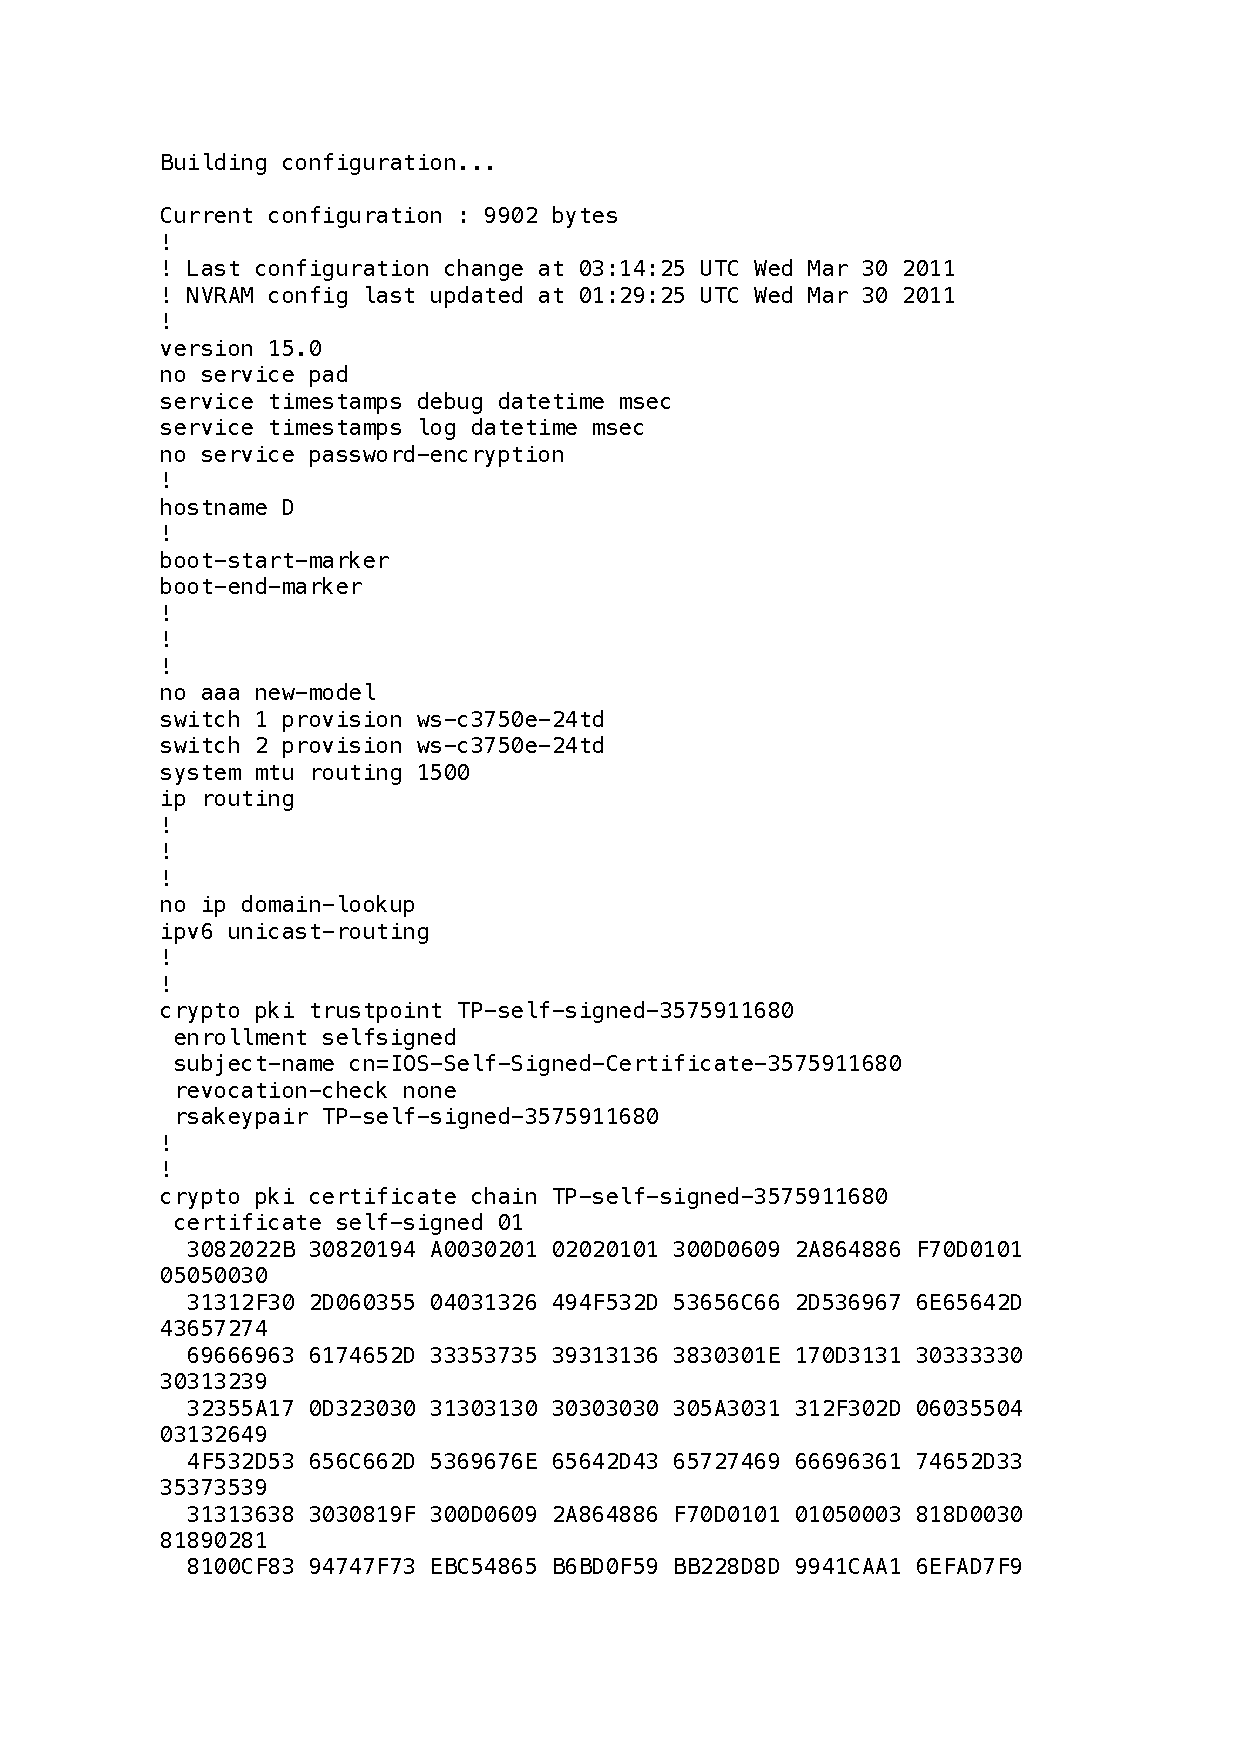
\includegraphics[height=\dimexpr\textheight-4\baselineskip\relax,page=1]{../config_files/D.pdf}
\includepdf[pagecommand={\thispagestyle{headings}},pages=2-]{../config_files/D.pdf}

\section{A1}
\vspace{-1cm}
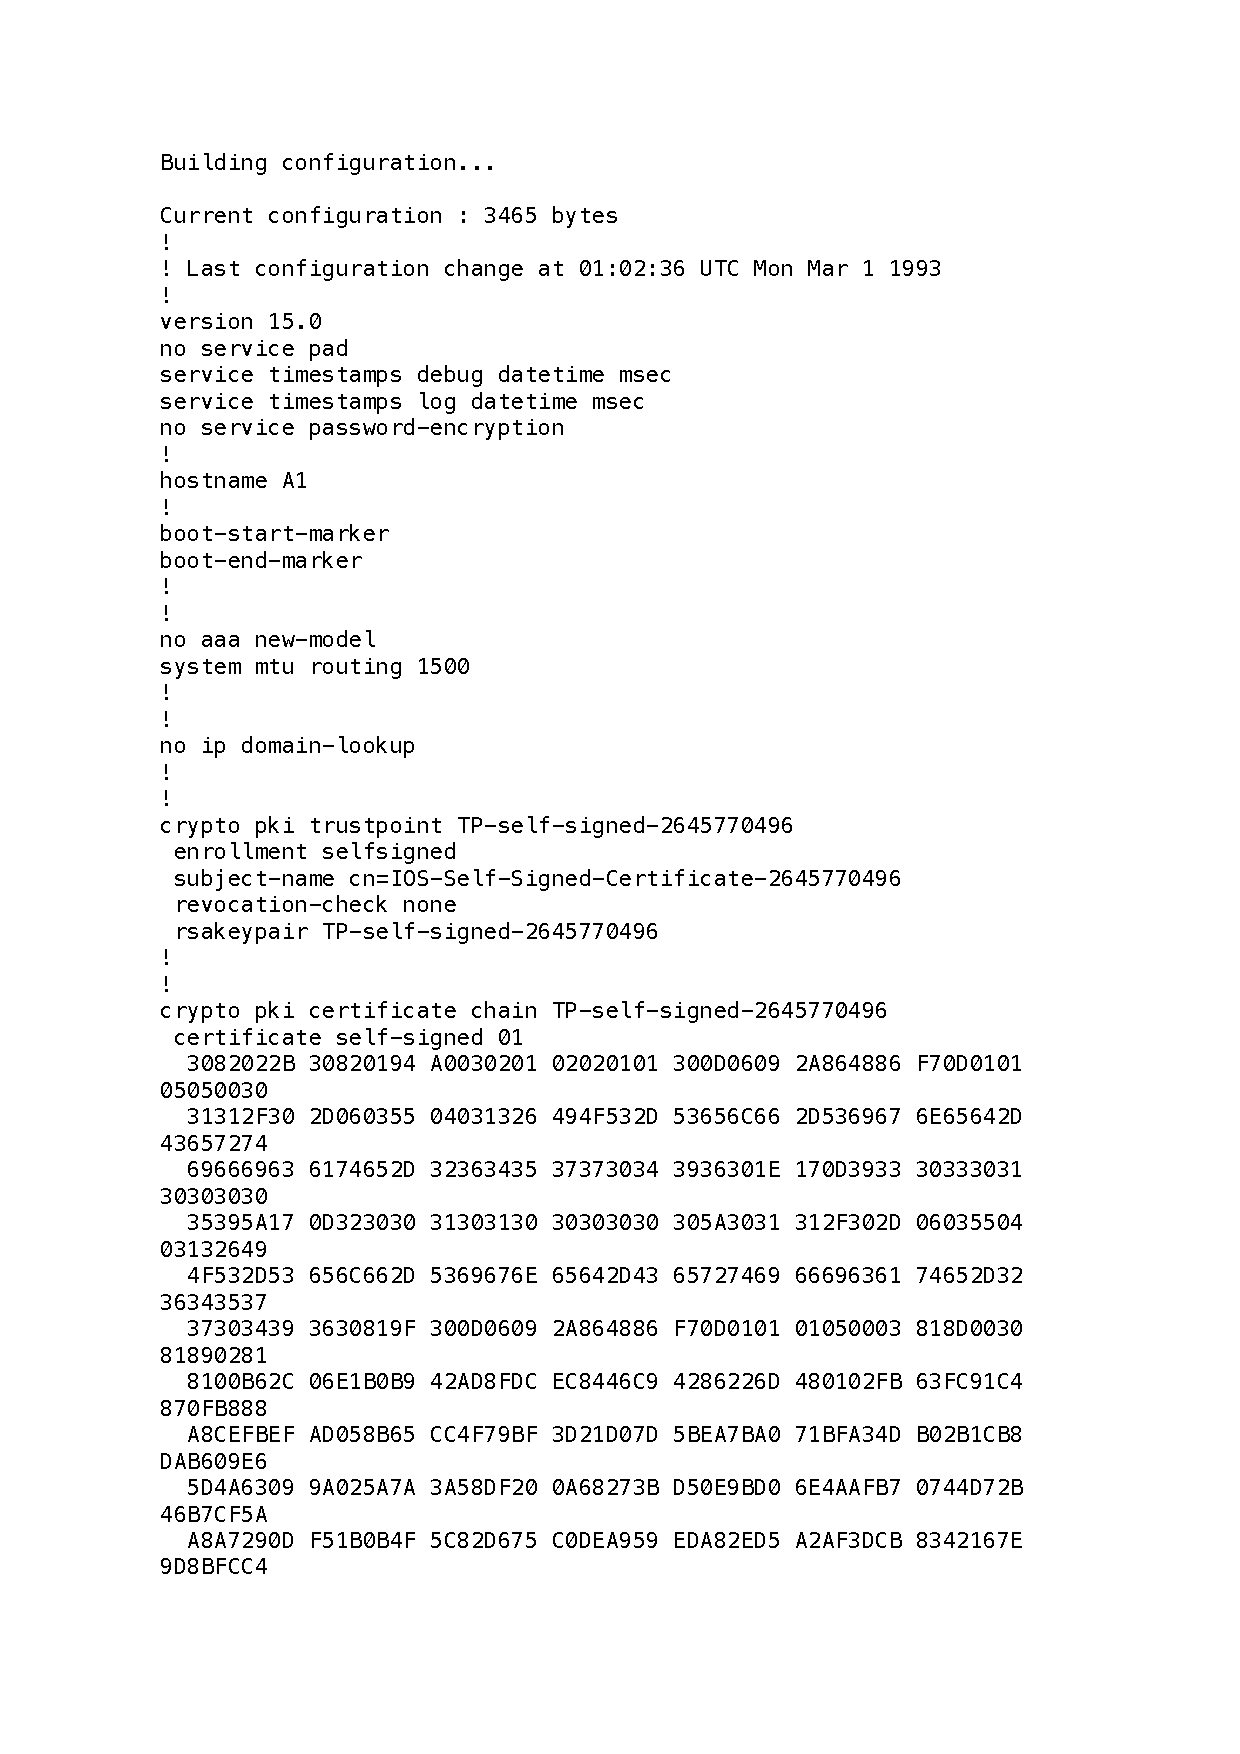
\includegraphics[height=\dimexpr\textheight-4\baselineskip\relax,page=1]{../config_files/A1.pdf}
\includepdf[pagecommand={\thispagestyle{headings}},pages=2-]{../config_files/A1.pdf}

\section{A2}
\vspace{-1cm}
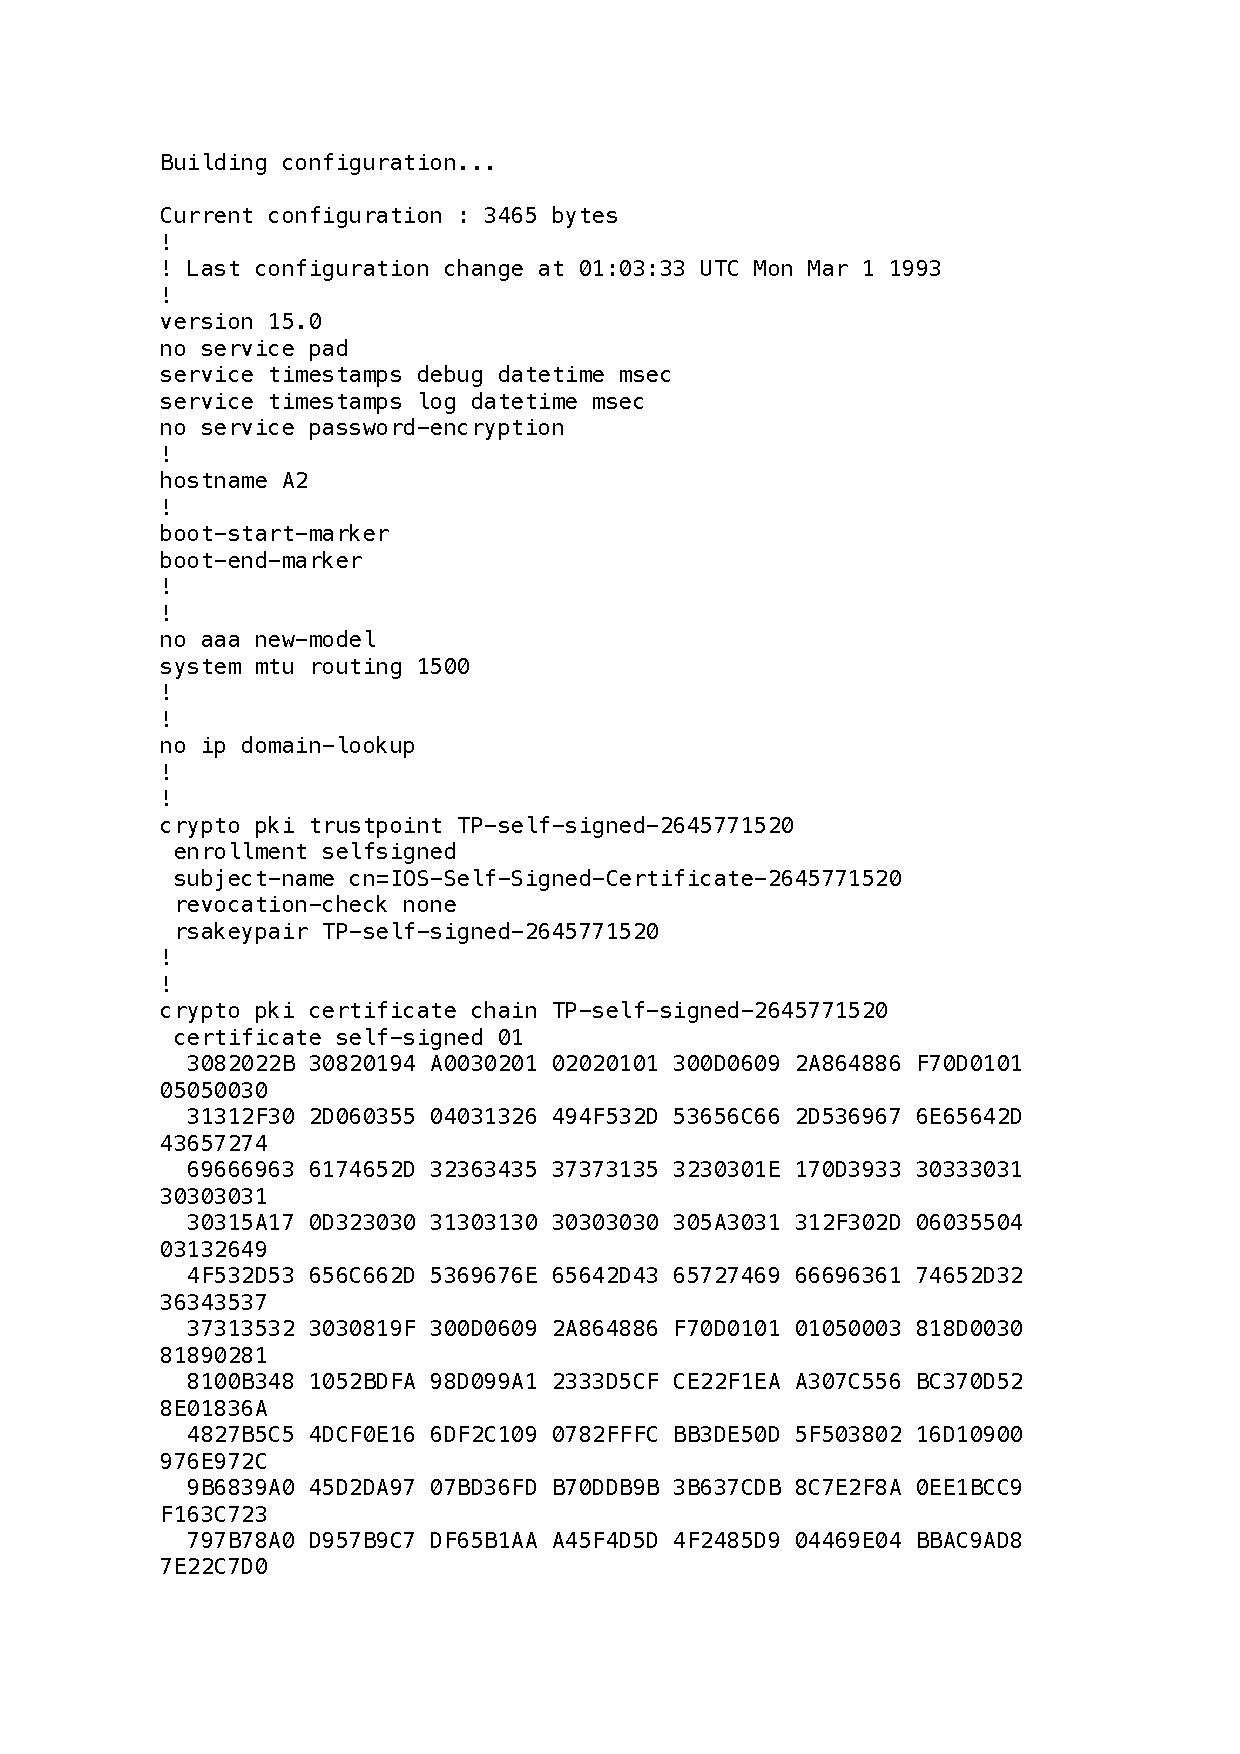
\includegraphics[height=\dimexpr\textheight-4\baselineskip\relax,page=1]{../config_files/A2.pdf}
\includepdf[pagecommand={\thispagestyle{headings}},pages=2-]{../config_files/A2.pdf}

\section{S1}
\vspace{-1cm}
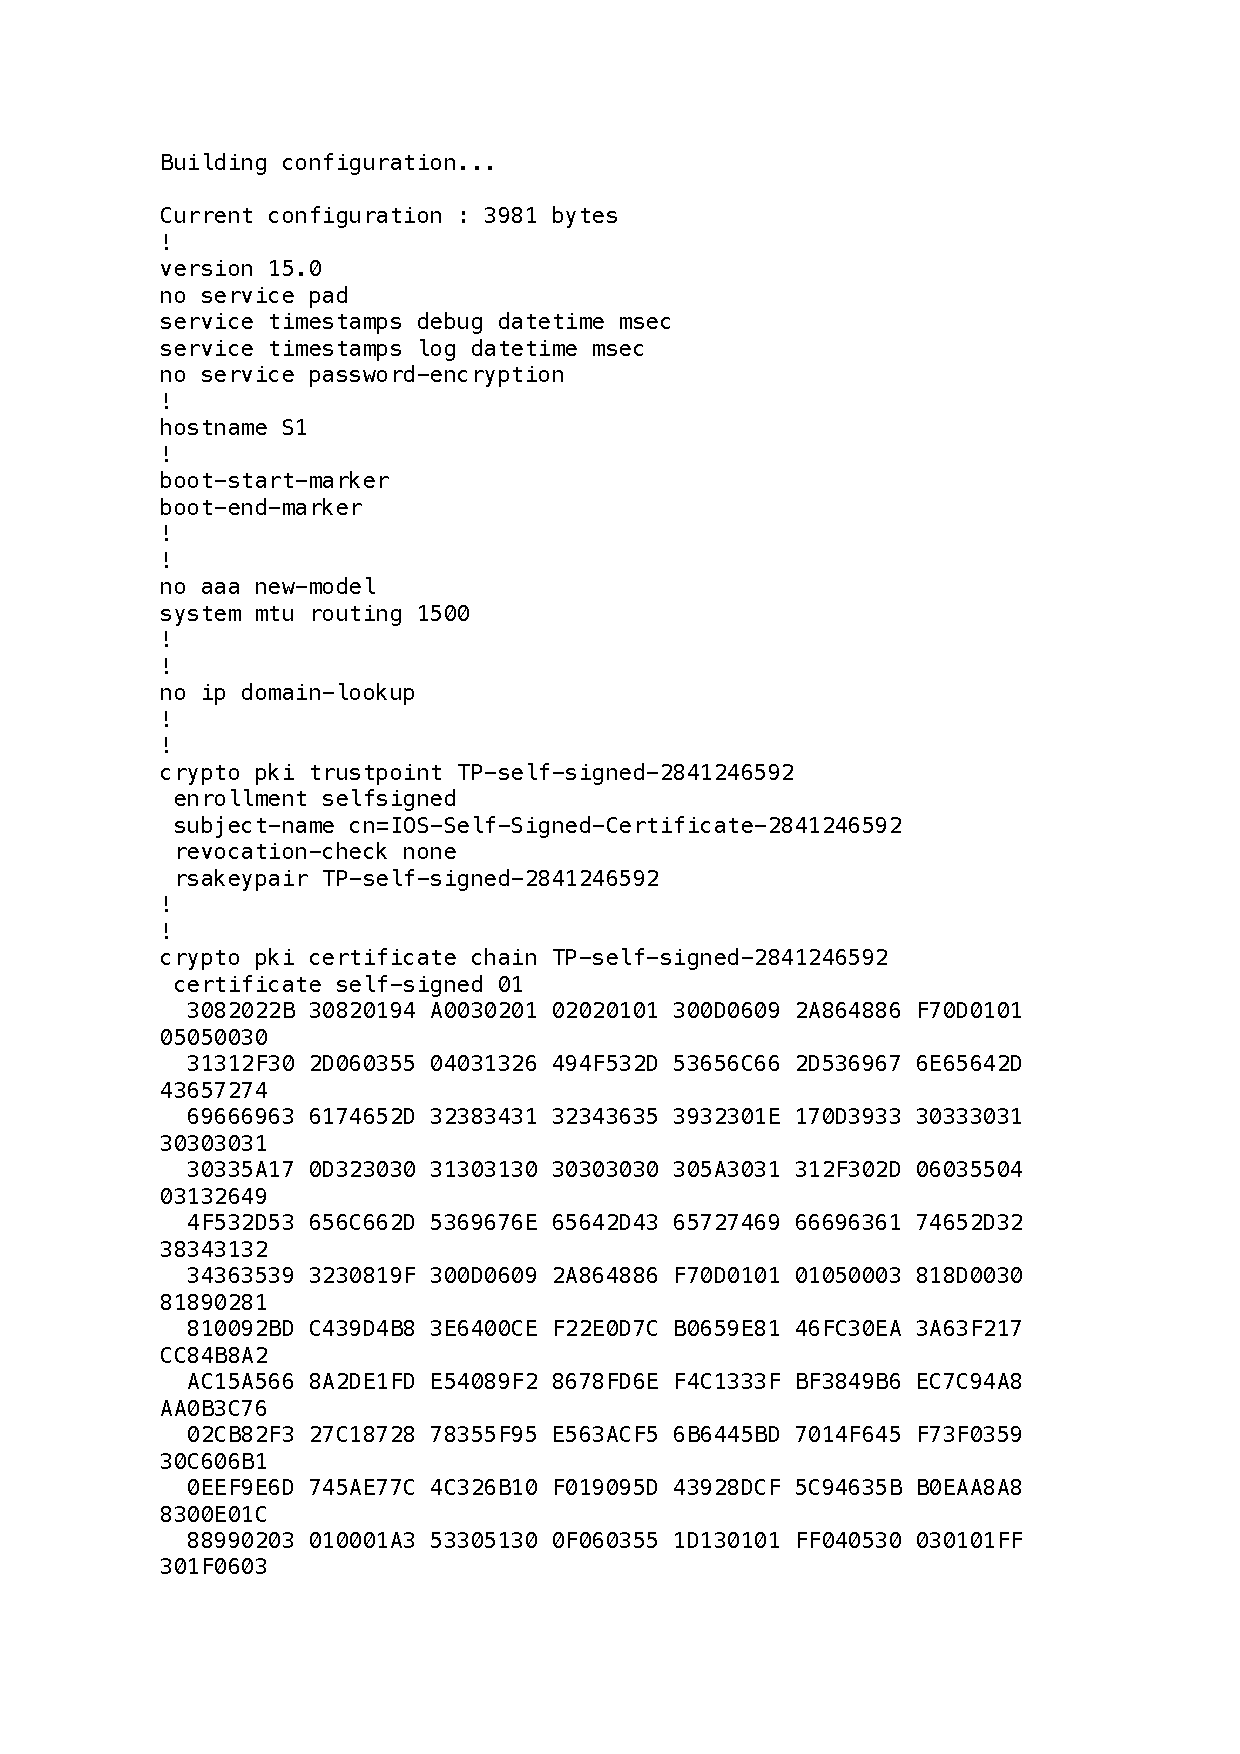
\includegraphics[height=\dimexpr\textheight-4\baselineskip\relax,page=1]{../config_files/S1.pdf}
\includepdf[pagecommand={\thispagestyle{headings}},pages=2-]{../config_files/S1.pdf}

\section{S2}
\vspace{-1cm}
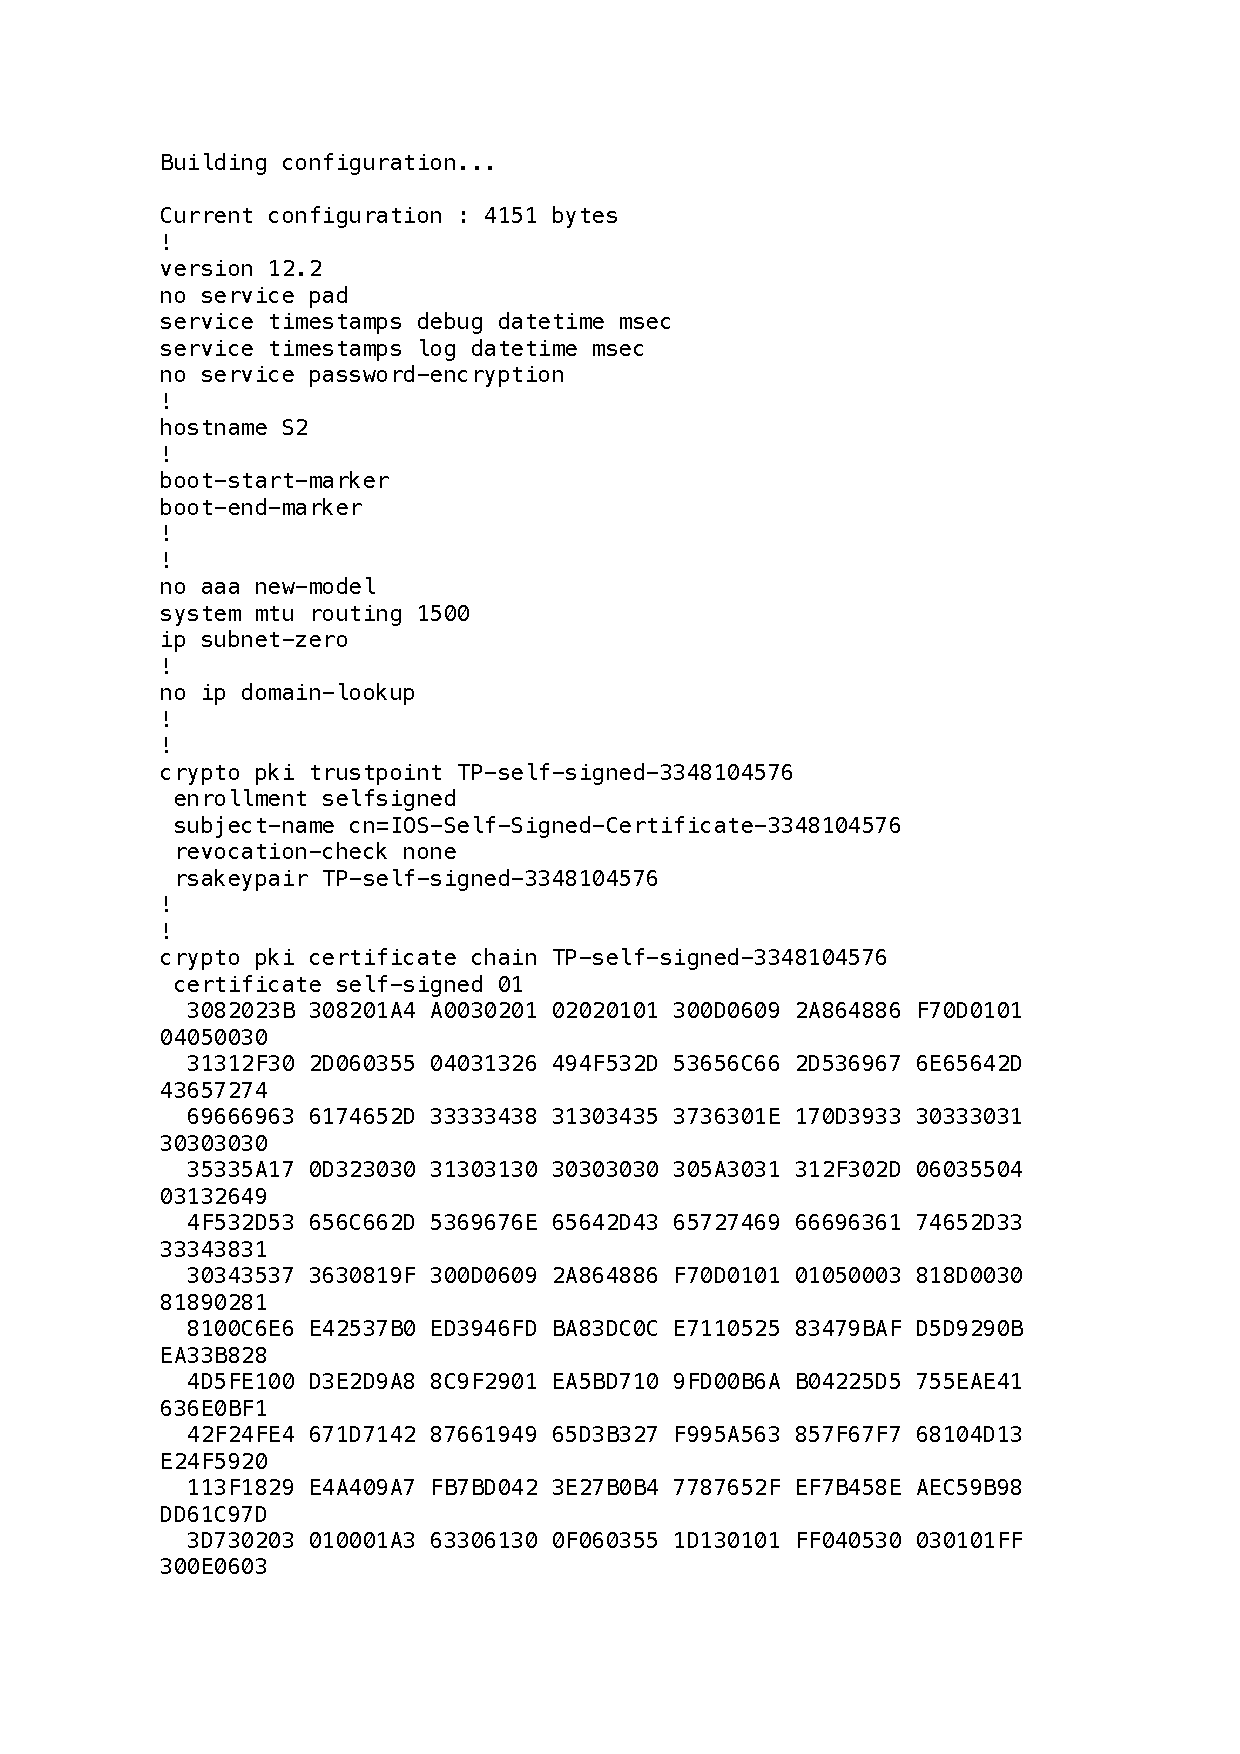
\includegraphics[height=\dimexpr\textheight-4\baselineskip\relax,page=1]{../config_files/S2.pdf}
\includepdf[pagecommand={\thispagestyle{headings}},pages=2-]{../config_files/S2.pdf}


\end{document}









